% !TEX program = pdflatex
% !TEX root = resume.tex
\documentclass[10pt,a4paper]{article}

% =========================================================
% BEATRIZ VOCURCA FRADE
% ATS / AI FRIENDLY BILINGUAL RESUME
% Updated: September 2026
%
% One source, several PDFs (see build.sh):
%   \CVLang = both | en | pt   (bilingual, English only, Portuguese only)
%
%   pdflatex resume.tex                  -> bilingual
%   pdflatex -jobname=X "\def\CVLang{en}% !TEX program = pdflatex
% !TEX root = resume.tex
\documentclass[10pt,a4paper]{article}

% =========================================================
% BEATRIZ VOCURCA FRADE
% ATS / AI FRIENDLY BILINGUAL RESUME
% Updated: September 2026
%
% One source, several PDFs (see build.sh):
%   \CVLang = both | en | pt   (bilingual, English only, Portuguese only)
%
%   pdflatex resume.tex                  -> bilingual
%   pdflatex -jobname=X "\def\CVLang{en}% !TEX program = pdflatex
% !TEX root = resume.tex
\documentclass[10pt,a4paper]{article}

% =========================================================
% BEATRIZ VOCURCA FRADE
% ATS / AI FRIENDLY BILINGUAL RESUME
% Updated: September 2026
%
% One source, several PDFs (see build.sh):
%   \CVLang = both | en | pt   (bilingual, English only, Portuguese only)
%
%   pdflatex resume.tex                  -> bilingual
%   pdflatex -jobname=X "\def\CVLang{en}% !TEX program = pdflatex
% !TEX root = resume.tex
\documentclass[10pt,a4paper]{article}

% =========================================================
% BEATRIZ VOCURCA FRADE
% ATS / AI FRIENDLY BILINGUAL RESUME
% Updated: September 2026
%
% One source, several PDFs (see build.sh):
%   \CVLang = both | en | pt   (bilingual, English only, Portuguese only)
%
%   pdflatex resume.tex                  -> bilingual
%   pdflatex -jobname=X "\def\CVLang{en}\input{resume}"
% =========================================================

\providecommand{\CVLang}{both}

% =========================================================
% PACKAGES
% =========================================================
\usepackage[
    top=0.85cm,
    bottom=0.85cm,
    left=1.15cm,
    right=1.15cm
]{geometry}

\usepackage[T1]{fontenc}
\usepackage[utf8]{inputenc}
% Source Sans Pro ships with TeX Live / Overleaf (lmodern is not installed
% on every machine, which broke the build).
\usepackage[default,lining]{sourcesanspro}
\usepackage{microtype}
\usepackage{xcolor}
\usepackage{graphicx}
\usepackage{fontawesome5}
\usepackage{enumitem}
\usepackage{tabularx}
\usepackage{array}
\usepackage{hyperref}
\usepackage{ragged2e}
\usepackage{needspace}
\usepackage{ifthen}

% Improves PDF text extraction for ATS / AI systems
\input{glyphtounicode}
\pdfgentounicode=1

% ATS: icons are decorative. Map every icon glyph to a plain space so text
% extractors never emit stray characters next to contact details or headings.
\pdfglyphtounicode{map-marker}{0020}
\pdfglyphtounicode{map-marker-alt}{0020}
\pdfglyphtounicode{laptop}{0020}
\pdfglyphtounicode{phone}{0020}
\pdfglyphtounicode{envelope}{0020}
\pdfglyphtounicode{linkedin}{0020}
\pdfglyphtounicode{github}{0020}
\pdfglyphtounicode{user}{0020}
\pdfglyphtounicode{code}{0020}
\pdfglyphtounicode{briefcase}{0020}
\pdfglyphtounicode{graduation-cap}{0020}
\pdfglyphtounicode{certificate}{0020}

% ATS: write real space characters into the PDF text layer, so parsers never
% glue words at font changes ("inFlutter"), which breaks keyword matching.
\pdfinterwordspaceon

% =========================================================
% GLOBAL CONFIGURATION
% =========================================================
\pagestyle{empty}

\setlength{\parindent}{0pt}
\setlength{\parskip}{0pt}

\renewcommand{\familydefault}{\sfdefault}

% \justifying (ragged2e) would otherwise indent every new paragraph
\setlength{\JustifyingParindent}{0pt}

\clubpenalty=10000
\widowpenalty=10000

% ATS: never hyphenate, so keywords are never split across lines.
\hyphenpenalty=10000
\exhyphenpenalty=10000
\emergencystretch=2em

% =========================================================
% COLORS
% =========================================================
\definecolor{primary}{HTML}{223846}
\definecolor{accent}{HTML}{3F6678}
\definecolor{muted}{HTML}{66747D}
\definecolor{text}{HTML}{20252A}
\definecolor{line}{HTML}{CDD7DC}
\definecolor{soft}{HTML}{F3F6F7}
\definecolor{white}{HTML}{FFFFFF}

% =========================================================
% PERSONAL INFORMATION
% =========================================================
\newcommand{\FullName}{Beatriz Vocurca Frade}

\newcommand{\Email}
{beatrizvocurcafrade@gmail.com}

\newcommand{\LinkedInURL}
{https://www.linkedin.com/in/beatriz-mobile/}

\newcommand{\LinkedInText}
{linkedin.com/in/beatriz-mobile}

\newcommand{\GitHubURL}
{https://github.com/BeatrizVocurcaFrade}

\newcommand{\GitHubText}
{github.com/BeatrizVocurcaFrade}

\newcommand{\LocationEN}
{Belo Horizonte, Minas Gerais, Brazil}

\newcommand{\LocationPT}
{Belo Horizonte, Minas Gerais, Brasil}

\newcommand{\WorkModeEN}
{Remote (UTC-3) · available immediately}

\newcommand{\WorkModePT}
{Remoto ou híbrido em BH · disponibilidade imediata}

% =========================================================
% PDF / LINKS
% =========================================================
\hypersetup{
    colorlinks=true,
    urlcolor=accent,
    linkcolor=accent,
    pdfauthor={Beatriz Vocurca Frade},
    pdfkeywords={
        Flutter,
        Dart,
        Flutter Developer,
        Mobile Developer,
        Mobile Software Engineer,
        Software Engineer,
        Mobile Engineer,
        Android,
        iOS,
        BLoC,
        Cubit,
        Freezed,
        GoRouter,
        Flavors,
        White-label,
        Platform Channels,
        Kotlin,
        Swift,
        In-App Purchases,
        Firebase,
        Crashlytics,
        Analytics,
        Firebase Realtime Database,
        Feature Flags,
        REST API,
        REST APIs,
        API Integration,
        Protobuf,
        WebSocket,
        JSON,
        React,
        React Native,
        TypeScript,
        NestJS,
        Prisma,
        PostgreSQL,
        Java,
        Spring,
        SQL,
        Clean Architecture,
        Clean Code,
        SOLID,
        Design Patterns,
        Git,
        GitHub,
        GitHub Actions,
        Codemagic,
        Azure DevOps,
        CI/CD,
        Figma,
        Swagger,
        Automated Testing,
        Unit Testing,
        Widget Testing,
        Code Review,
        Refactoring,
        Debugging,
        Performance,
        Agile,
        Scrum,
        Kanban,
        Football,
        Sports Data,
        Live Sports,
        Football Statistics
    }
}

\urlstyle{same}

% =========================================================
% LIST CONFIGURATION
% =========================================================
\setlist[itemize]{
    leftmargin=0.43cm,
    itemsep=0.035cm,
    topsep=0.055cm,
    parsep=0pt,
    partopsep=0pt
}

% =========================================================
% SECTION
% =========================================================
\newcommand{\cvsection}[2]{

    \needspace{4\baselineskip}

    \vspace{0.18cm}

    {\large
    \bfseries
    \color{primary}
    #1
    \hspace{0.10cm}
    #2}

    \vspace{0.025cm}

    {\color{line}
    \rule{\linewidth}{0.65pt}}

    \vspace{0.07cm}
}

% =========================================================
% EXPERIENCE
% =========================================================
\newcommand{\experience}[4]{

    \needspace{5\baselineskip}

    \begin{tabularx}{\linewidth}{
        @{}
        >{\raggedright\arraybackslash}X
        >{\raggedleft\arraybackslash}p{3.25cm}
        @{}
    }

    {\bfseries\color{text}#1}
    &
    {\small\bfseries\color{accent}#3}
    \\[-0.01cm]
    {\small
    \bfseries
    \color{muted}
    #2}
    &
    \end{tabularx}

    \vspace{-0.09cm}

    {\small
    \color{text}
    #4
    }

    \vspace{0.07cm}
}

% =========================================================
% EDUCATION
% =========================================================
\newcommand{\education}[4]{

    \needspace{3\baselineskip}

    \begin{tabularx}{\linewidth}{
        @{}
        >{\raggedright\arraybackslash}X
        >{\raggedleft\arraybackslash}p{3.1cm}
        @{}
    }

    {\bfseries\color{text}#1}
    &
    {\small\bfseries\color{accent}#3}
    \\[-0.01cm]
    {\small\color{muted}#2}
    &
    \end{tabularx}

    \ifthenelse{\equal{#4}{}}
    {}
    {
        {\small\color{text}#4}
    }

    \vspace{0.09cm}
}

% =========================================================
% SKILL LINE
% =========================================================
\newcommand{\skillline}[2]{
    {\small
    \textbf{\color{primary}#1:}
    \color{text}
    #2
    }

    \vspace{0.045cm}
}

% =========================================================
% HEADER
%
% #1 title, #2 keyword line, #3 location, #4 photo | nophoto, #5 work mode
% (the English version omits the photo, as most international
% recruiters expect; the Portuguese version keeps it)
% =========================================================
\newcommand{\HeaderName}[2]{
    {\fontsize{24}{27}\selectfont
    \bfseries
    \color{primary}
    \FullName}

    \vspace{0.045cm}

    {\normalsize
    \bfseries
    \color{accent}
    #1}

    \vspace{0.055cm}

    {\small
    \color{muted}
    #2}
}

\newcommand{\HeaderContacts}[2]{
    {\small
    \color{text}

    \faMapMarker
    \hspace{0.045cm}
    #1

    \par\vspace{0.08cm}

    \faLaptop
    \hspace{0.045cm}
    #2

    \par\vspace{0.08cm}

    \faEnvelope
    \hspace{0.045cm}
    \href{mailto:\Email}{\Email}

    \par\vspace{0.08cm}

    \faLinkedin
    \hspace{0.045cm}
    \href{\LinkedInURL}{\LinkedInText}

    \par\vspace{0.08cm}

    \faGithub
    \hspace{0.045cm}
    \href{\GitHubURL}{\GitHubText}

    }
}

\newcommand{\CVHeader}[5]{

    \noindent
    \ifthenelse{\equal{#4}{photo}}
    {
        \begin{tabularx}{\linewidth}{
            @{}
            >{\raggedright\arraybackslash}X
            >{\centering\arraybackslash}p{4.45cm}
            @{}
        }

        \begin{minipage}[c]{\linewidth}

            \HeaderName{#1}{#2}

            \vspace{0.15cm}

            \HeaderContacts{#3}{#5}

        \end{minipage}

        &

        % PROFILE PHOTO (profile.jpg next to this file)
        \begin{minipage}[c]{4.35cm}

            \centering

            \IfFileExists{profile.jpg}
            {
                \fcolorbox{line}{white}{%
                    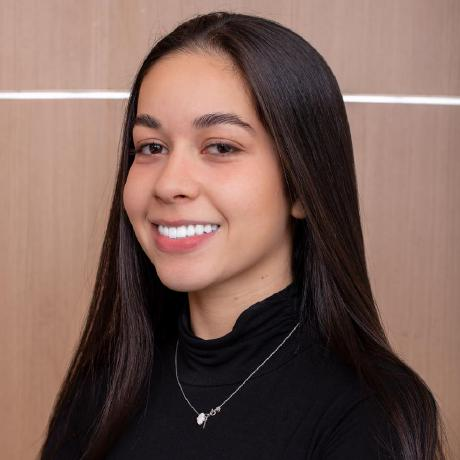
\includegraphics[
                        width=4.20cm,
                        height=4.20cm,
                        keepaspectratio
                    ]{profile.jpg}%
                }
            }
            {
                \fcolorbox{line}{soft}{
                    \parbox[c][4.20cm][c]{4.20cm}{
                        \centering

                        \color{muted}

                        \Large
                        \faUser

                        \par\vspace{0.10cm}

                        \scriptsize
                        profile.jpg
                    }
                }
            }

        \end{minipage}

        \end{tabularx}
    }
    {
        \begin{tabularx}{\linewidth}{
            @{}
            >{\raggedright\arraybackslash}X
            >{\raggedright\arraybackslash}p{6.2cm}
            @{}
        }

        \begin{minipage}[c]{\linewidth}

            \HeaderName{#1}{#2}

        \end{minipage}

        &

        \begin{minipage}[c]{\linewidth}

            \HeaderContacts{#3}{#5}

        \end{minipage}

        \end{tabularx}
    }

    \vspace{0.10cm}

    {\color{primary}
    \rule{\linewidth}{1.15pt}}

    \vspace{0.10cm}
}

% =========================================================
% COMPANY DESCRIPTOR (one line of context under a role)
% =========================================================
\newcommand{\roleinfo}[1]{
    {\small\itshape\color{muted}#1}

    \vspace{-0.03cm}
}

% =========================================================
% =========================================================
% ENGLISH VERSION
% =========================================================
% =========================================================

\newcommand{\EnglishCV}{

% =========================================================
% HEADER
% =========================================================
\CVHeader
{MOBILE SOFTWARE ENGINEER \;|\; FLUTTER DEVELOPER}
{Flutter \;•\; Dart \;•\; Android \& iOS \;•\; 4+ years in production}
{\LocationEN}
{nophoto}
{\WorkModeEN}

% =========================================================
% SUMMARY
% =========================================================
\cvsection{\faUser}{Professional Summary}

{\small
\justifying
Mobile Software Engineer specialized in \textbf{Flutter and Dart}, with 4+
years shipping production apps for Android and iOS and a B.Sc. in Systems
Engineering from UFMG. At \textbf{R10 Score} (1M+ Google Play downloads),
built real-time, high-traffic features end to end, such as the 2026 World Cup
experience and the live bet wall. At Prime Results, turned a white-label app
for 8 client companies into one flavor-based codebase. Strong in
Clean Architecture, BLoC/Cubit, real-time data (WebSocket, Protobuf) and testing;
also delivers with React, NestJS, Java and Spring.
}

% =========================================================
% CORE SKILLS
% =========================================================
\cvsection{\faCode}{Core Technical Skills}

\skillline
{Mobile}
{Flutter, Dart, Android, iOS, Kotlin, Swift, platform channels, flavors /
white-label, adaptive tablet UI, In-App Purchases, React Native}

\skillline
{State \& Architecture}
{BLoC, Cubit, Freezed, GoRouter, Clean Architecture, SOLID, dependency
injection, modular monorepo}

\skillline
{APIs \& Real-Time}
{REST APIs, JSON, Protobuf, WebSocket, Swagger / OpenAPI}

\skillline
{Firebase \& Data}
{Firebase, Crashlytics, Analytics, Realtime Database, feature flags, SQL,
PostgreSQL}

\skillline
{Web \& Backend}
{React, TypeScript, NestJS, Prisma, Java, Spring}

\skillline
{Quality \& Delivery}
{Unit, Widget \& Integration Testing (bloc\_test, mocktail), Code Review, CI/CD, GitHub
Actions, Codemagic, Git, Azure DevOps, Figma, Scrum, AI-assisted development
(Claude Code)}

\skillline
{Languages}
{Portuguese (native), English (professional working proficiency, B2 · TOEFL)}

% =========================================================
% EXPERIENCE
% =========================================================
\cvsection{\faBriefcase}{Professional Experience}

\experience
{Full Stack Developer | Mobile (Flutter)}
{OTG Ventures \;·\; R10 Score}
{Jun 2025 -- Sep 2026}
{
\roleinfo{Live football scores and statistics app \;·\; 1M+ Google
Play downloads \;·\; 11-package Flutter
monorepo}

\begin{itemize}

    \item
    Delivered the \textbf{2026 World Cup experience} (bracket, group tables,
    Favorite Team vote, match guesses and CMS-driven content) in time for the
    tournament's fixed start, joined by
    \textbf{22\% of all accounts}.

    \item
    Main mobile developer on \textbf{Notified Bet}: a live bet wall with
    drag-and-drop ordering saved on the backend (optimistic updates with
    rollback) and live status over \textbf{WebSocket}.

    \item
    \textbf{Unblocked Google Play publishing} after the 2026 target-API
    deadline (targetSdk 36, Play Billing Library 8.0.0), protecting In-App
    Purchase subscription revenue.

    \item
    Brought the test suite back to green, fixing two production bugs along the
    way, and tracked down an intermittent freeze in match statistics; one of
    the team's most active contributors, with \textbf{500+ merged PRs} and
    570+ code reviews.

    \item
    Built on \textbf{WebSocket (Protobuf and JSON) and REST}, with
    \textbf{Firebase} feature flags and Crashlytics; also contributed full stack
    to \textbf{OTG Partners}, the group's affiliate-commission platform
    (\textbf{React, NestJS}, Prisma, PostgreSQL).
\end{itemize}
}

\experience
{Mobile Developer}
{Prime Results}
{May 2022 -- May 2025}
{
\roleinfo{Intern from May 2022, Mobile Developer from Feb 2023 \;·\; white-label app for the
field and point-of-sale teams of 8 client companies \;·\; Android \& iOS}

\begin{itemize}

    \item
    Consolidated a \textbf{white-label app for 8 client companies}, kept on
    separate cherry-picked branches, into \textbf{one codebase with Flutter
    flavors}, so every fix ships to all clients from a single main branch.

    \item
    Adjusted and improved \textbf{phone and tablet layouts} across the app,
    used by field and point-of-sale teams.

    \item
    Delivered features end to end, from \textbf{Figma} to \textbf{REST API}
    integration and releases on \textbf{Google Play and the App Store}, and contributed to \textbf{Java and Spring}
    services and \textbf{React} web projects.
\end{itemize}
}

\experience
{Mobile Developer -- Freelance}
{Upbeat Studio \;·\; Drum Coach app -- Germany (remote)}
{Mar 2025 -- Apr 2025}
{
\begin{itemize}

    \item
    Built an interactive \textbf{Flutter and Dart} app for learning and
    practicing drums, working remotely and autonomously with an international
    team in English.
\end{itemize}
}

\experience
{Programming Instructor (Volunteer)}
{Garotas Aplicadas Project -- AVEC | Centro Universitário Una}
{Jan 2025 -- Aug 2026}
{
\begin{itemize}

    \item
    Taught theory and hands-on programming classes to public
    high-school girls in Belo Horizonte, in a social initiative to
    widen female participation in technology.
\end{itemize}
}

\experience
{Business Analyst \& Front-End Developer}
{iJunior}
{Mar 2022 -- May 2022}
{
\begin{itemize}

    \item
    Gathered requirements with clients and the sales team and built custom
    apps and websites with \textbf{React Native} for organizations across
    different sectors, using \textbf{Scrum and Kanban}.
\end{itemize}
}

\experience
{Systems Analyst}
{Interact Place}
{Oct 2021 -- Jan 2022}
{
\begin{itemize}

    \item
    Helped build an interactive mobile exhibition guide for
    \textbf{Palácio das Artes}, one of Belo Horizonte's major cultural
    institutions, where QR codes connect visitors to artwork information.
\end{itemize}
}

% =========================================================
% EDUCATION
% =========================================================
\cvsection{\faGraduationCap}{Education \& Certifications}

\education
{Bachelor's Degree in Systems Engineering}
{Federal University of Minas Gerais -- UFMG}
{2020 -- 2026}
{}

\skillline
{Certifications}
{TOEFL (English, B2) \;·\; CCAA English course (2008 -- 2019) \;·\; Google
Play Academy -- Store Listing Certificate}

}


% =========================================================
% =========================================================
% PORTUGUESE VERSION
% =========================================================
% =========================================================

\newcommand{\PortugueseCV}{

% =========================================================
% HEADER
% =========================================================
\CVHeader
{ENGENHEIRA DE SOFTWARE MOBILE \;|\; DESENVOLVEDORA FLUTTER}
{Flutter \;•\; Dart \;•\; Android e iOS \;•\; 4+ anos em produção}
{\LocationPT}
{photo}
{\WorkModePT}

% =========================================================
% SUMMARY
% =========================================================
\cvsection{\faUser}{Resumo Profissional}

{\small
\justifying
Engenheira de Software Mobile especializada em \textbf{Flutter e Dart}, com
mais de 4 anos entregando apps em produção para Android e iOS, formada em
Engenharia de Sistemas pela UFMG. No \textbf{R10 Score} (mais de 1 milhão de
downloads no Google Play), desenvolvi de ponta a ponta funcionalidades em tempo
real e de alto tráfego, como a experiência da Copa do Mundo 2026 e o mural de
apostas ao vivo. Na Prime Results, transformei um app white-label de 8 empresas
clientes em um único código com flavors. Forte em Clean Architecture,
BLoC/Cubit, dados em tempo real (WebSocket, Protobuf) e testes; também atuo com
React, NestJS, Java e Spring.
}

% =========================================================
% CORE SKILLS
% =========================================================
\cvsection{\faCode}{Competências Técnicas}

\skillline
{Mobile}
{Flutter, Dart, Android, iOS, Kotlin, Swift, platform channels, flavors /
white-label, UI adaptativa para tablet, compras in-app, React Native}

\skillline
{Estado \& Arquitetura}
{BLoC, Cubit, Freezed, GoRouter, Clean Architecture, SOLID, injeção de
dependência, monorepo modular}

\skillline
{APIs \& Tempo Real}
{APIs REST, JSON, Protobuf, WebSocket, Swagger / OpenAPI}

\skillline
{Firebase \& Dados}
{Firebase, Crashlytics, Analytics, Realtime Database, feature flags, SQL,
PostgreSQL}

\skillline
{Web \& Backend}
{React, TypeScript, NestJS, Prisma, Java, Spring}

\skillline
{Qualidade \& Entrega}
{Testes Unitários, de Widget e de Integração (bloc\_test, mocktail), Code Review, CI/CD,
GitHub Actions, Codemagic, Git, Azure DevOps, Figma, Scrum, desenvolvimento
assistido por IA (Claude Code)}

\skillline
{Idiomas}
{Português (nativo), Inglês (proficiência profissional, B2 · TOEFL)}

% =========================================================
% EXPERIENCE
% =========================================================
\cvsection{\faBriefcase}{Experiência Profissional}

\experience
{Desenvolvedora Full Stack | Mobile (Flutter)}
{OTG Ventures \;·\; R10 Score}
{Jun 2025 -- Set 2026}
{
\roleinfo{App de placares e estatísticas de futebol ao vivo \;·\;
mais de 1 milhão de downloads no Google Play \;·\; monorepo Flutter com 11 pacotes}

\begin{itemize}

    \item
    Entreguei a \textbf{experiência da Copa do Mundo 2026} (chaveamento,
    tabela de grupos, votação do Time do Coração, palpites e conteúdo via CMS)
    a tempo do início do torneio, com adesão de
    \textbf{22\% de todas as contas}.

    \item
    Principal desenvolvedora mobile da \textbf{Aposta Notificada}: mural de apostas ao vivo
    com reordenação por drag-and-drop salva no backend (atualização otimista
    com rollback) e status em tempo real via \textbf{WebSocket}.

    \item
    \textbf{Desbloqueei a publicação no Google Play} após o prazo de target
    API de 2026 (targetSdk 36, Play Billing Library 8.0.0), protegendo a
    receita das assinaturas (compras in-app).

    \item
    Recuperei a suíte de testes, corrigindo dois bugs de produção no caminho,
    e rastreei um travamento intermitente nas estatísticas das partidas; estou
    entre as pessoas mais ativas do time, com \textbf{mais de 500 PRs}
    mergeados e mais de 570 code reviews.

    \item
    Desenvolvi sobre \textbf{WebSocket (Protobuf e JSON) e REST}, com
    feature flags no \textbf{Firebase} e Crashlytics; atuei também full stack
    no \textbf{OTG Partners}, plataforma de comissões de afiliados do grupo
    (\textbf{React, NestJS}, Prisma, PostgreSQL).
\end{itemize}
}

\experience
{Desenvolvedora Mobile}
{Prime Results}
{Mai 2022 -- Mai 2025}
{
\roleinfo{Estagiária desde mai 2022, Desenvolvedora Mobile desde fev 2023 \;·\; app
white-label para equipes de campo e de ponto de venda de 8 empresas clientes}

\begin{itemize}

    \item
    Consolidei um \textbf{app white-label de 8 empresas clientes}, mantido em
    branches separadas sincronizadas por cherry-pick, em \textbf{um único
    código com flavors do Flutter}, para que cada correção chegue a todos os
    clientes a partir de uma única branch principal.

    \item
    Ajustei e melhorei \textbf{layouts para celular e tablet} em todo o app,
    usado por equipes de campo e de ponto de venda.

    \item
    Entreguei funcionalidades de ponta a ponta, do \textbf{Figma} à
    integração com \textbf{APIs REST} e à publicação no \textbf{Google Play e na App Store}, e contribuí em serviços
    \textbf{Java e Spring} e em projetos web com \textbf{React}.
\end{itemize}
}

\experience
{Desenvolvedora Mobile -- Freelancer}
{Upbeat Studio \;·\; app Drum Coach -- Alemanha (remoto)}
{Mar 2025 -- Abr 2025}
{
\begin{itemize}

    \item
    Desenvolvi um app interativo em \textbf{Flutter e Dart} para aprender e
    praticar bateria, em trabalho remoto e autônomo com uma equipe
    internacional, em inglês.
\end{itemize}
}

\experience
{Instrutora de Programação (Voluntária)}
{Projeto Garotas Aplicadas -- AVEC | Centro Universitário Una}
{Jan 2025 -- Ago 2026}
{
\begin{itemize}

    \item
    Dei aulas teóricas e práticas de programação para estudantes do ensino
    médio da rede pública de Belo Horizonte, em uma iniciativa social para
    ampliar a participação feminina na tecnologia.
\end{itemize}
}

\experience
{Analista de Negócios \& Desenvolvedora Front-End}
{iJunior}
{Mar 2022 -- Mai 2022}
{
\begin{itemize}

    \item
    Levantei requisitos com clientes e com a equipe comercial e desenvolvi
    aplicações e websites personalizados com \textbf{React Native} para
    organizações de diferentes segmentos, com \textbf{Scrum e Kanban}.
\end{itemize}
}

\experience
{Analista de Sistemas}
{Interact Place}
{Out 2021 -- Jan 2022}
{
\begin{itemize}

    \item
    Participei do desenvolvimento de um guia mobile interativo de exposições
    para o \textbf{Palácio das Artes}, uma das principais instituições
    culturais de Belo Horizonte, em que QR Codes conectam os visitantes a
    informações sobre as obras.
\end{itemize}
}

% =========================================================
% EDUCATION
% =========================================================
\cvsection{\faGraduationCap}{Formação \& Certificações}

\education
{Bacharelado em Engenharia de Sistemas}
{Universidade Federal de Minas Gerais -- UFMG}
{2020 -- 2026}
{}

\skillline
{Certificações}
{TOEFL (inglês, B2) \;·\; Curso de inglês CCAA (2008 -- 2019) \;·\; Google
Play Academy -- Store Listing Certificate}

}

% =========================================================
% LANGUAGE-SPECIFIC PDF METADATA
% =========================================================
\newcommand{\MetadataEN}{
    \hypersetup{
        pdftitle={Beatriz Vocurca Frade - Mobile Software Engineer - Flutter Developer},
        pdfsubject={Mobile Software Engineering, Flutter and Software Development Resume},
        pdflang={en-US}
    }
}

\newcommand{\MetadataPT}{
    \hypersetup{
        pdftitle={Beatriz Vocurca Frade - Engenheira de Software Mobile - Desenvolvedora Flutter},
        pdfsubject={Currículo de Engenharia de Software Mobile, Flutter e Desenvolvimento de Software},
        pdflang={pt-BR}
    }
}

\ifthenelse{\equal{\CVLang}{pt}}
{\MetadataPT}
{\MetadataEN}


% =========================================================
% DOCUMENT
% =========================================================
\begin{document}

\ifthenelse{\equal{\CVLang}{en}}
{
    \EnglishCV
}
{
    \ifthenelse{\equal{\CVLang}{pt}}
    {
        \PortugueseCV
    }
    {
        % Bilingual: English first, Portuguese after a page break
        \EnglishCV

        \newpage

        \PortugueseCV
    }
}

\end{document}
"
% =========================================================

\providecommand{\CVLang}{both}

% =========================================================
% PACKAGES
% =========================================================
\usepackage[
    top=0.85cm,
    bottom=0.85cm,
    left=1.15cm,
    right=1.15cm
]{geometry}

\usepackage[T1]{fontenc}
\usepackage[utf8]{inputenc}
% Source Sans Pro ships with TeX Live / Overleaf (lmodern is not installed
% on every machine, which broke the build).
\usepackage[default,lining]{sourcesanspro}
\usepackage{microtype}
\usepackage{xcolor}
\usepackage{graphicx}
\usepackage{fontawesome5}
\usepackage{enumitem}
\usepackage{tabularx}
\usepackage{array}
\usepackage{hyperref}
\usepackage{ragged2e}
\usepackage{needspace}
\usepackage{ifthen}

% Improves PDF text extraction for ATS / AI systems
\input{glyphtounicode}
\pdfgentounicode=1

% ATS: icons are decorative. Map every icon glyph to a plain space so text
% extractors never emit stray characters next to contact details or headings.
\pdfglyphtounicode{map-marker}{0020}
\pdfglyphtounicode{map-marker-alt}{0020}
\pdfglyphtounicode{laptop}{0020}
\pdfglyphtounicode{phone}{0020}
\pdfglyphtounicode{envelope}{0020}
\pdfglyphtounicode{linkedin}{0020}
\pdfglyphtounicode{github}{0020}
\pdfglyphtounicode{user}{0020}
\pdfglyphtounicode{code}{0020}
\pdfglyphtounicode{briefcase}{0020}
\pdfglyphtounicode{graduation-cap}{0020}
\pdfglyphtounicode{certificate}{0020}

% ATS: write real space characters into the PDF text layer, so parsers never
% glue words at font changes ("inFlutter"), which breaks keyword matching.
\pdfinterwordspaceon

% =========================================================
% GLOBAL CONFIGURATION
% =========================================================
\pagestyle{empty}

\setlength{\parindent}{0pt}
\setlength{\parskip}{0pt}

\renewcommand{\familydefault}{\sfdefault}

% \justifying (ragged2e) would otherwise indent every new paragraph
\setlength{\JustifyingParindent}{0pt}

\clubpenalty=10000
\widowpenalty=10000

% ATS: never hyphenate, so keywords are never split across lines.
\hyphenpenalty=10000
\exhyphenpenalty=10000
\emergencystretch=2em

% =========================================================
% COLORS
% =========================================================
\definecolor{primary}{HTML}{223846}
\definecolor{accent}{HTML}{3F6678}
\definecolor{muted}{HTML}{66747D}
\definecolor{text}{HTML}{20252A}
\definecolor{line}{HTML}{CDD7DC}
\definecolor{soft}{HTML}{F3F6F7}
\definecolor{white}{HTML}{FFFFFF}

% =========================================================
% PERSONAL INFORMATION
% =========================================================
\newcommand{\FullName}{Beatriz Vocurca Frade}

\newcommand{\Email}
{beatrizvocurcafrade@gmail.com}

\newcommand{\LinkedInURL}
{https://www.linkedin.com/in/beatriz-mobile/}

\newcommand{\LinkedInText}
{linkedin.com/in/beatriz-mobile}

\newcommand{\GitHubURL}
{https://github.com/BeatrizVocurcaFrade}

\newcommand{\GitHubText}
{github.com/BeatrizVocurcaFrade}

\newcommand{\LocationEN}
{Belo Horizonte, Minas Gerais, Brazil}

\newcommand{\LocationPT}
{Belo Horizonte, Minas Gerais, Brasil}

\newcommand{\WorkModeEN}
{Remote (UTC-3) · available immediately}

\newcommand{\WorkModePT}
{Remoto ou híbrido em BH · disponibilidade imediata}

% =========================================================
% PDF / LINKS
% =========================================================
\hypersetup{
    colorlinks=true,
    urlcolor=accent,
    linkcolor=accent,
    pdfauthor={Beatriz Vocurca Frade},
    pdfkeywords={
        Flutter,
        Dart,
        Flutter Developer,
        Mobile Developer,
        Mobile Software Engineer,
        Software Engineer,
        Mobile Engineer,
        Android,
        iOS,
        BLoC,
        Cubit,
        Freezed,
        GoRouter,
        Flavors,
        White-label,
        Platform Channels,
        Kotlin,
        Swift,
        In-App Purchases,
        Firebase,
        Crashlytics,
        Analytics,
        Firebase Realtime Database,
        Feature Flags,
        REST API,
        REST APIs,
        API Integration,
        Protobuf,
        WebSocket,
        JSON,
        React,
        React Native,
        TypeScript,
        NestJS,
        Prisma,
        PostgreSQL,
        Java,
        Spring,
        SQL,
        Clean Architecture,
        Clean Code,
        SOLID,
        Design Patterns,
        Git,
        GitHub,
        GitHub Actions,
        Codemagic,
        Azure DevOps,
        CI/CD,
        Figma,
        Swagger,
        Automated Testing,
        Unit Testing,
        Widget Testing,
        Code Review,
        Refactoring,
        Debugging,
        Performance,
        Agile,
        Scrum,
        Kanban,
        Football,
        Sports Data,
        Live Sports,
        Football Statistics
    }
}

\urlstyle{same}

% =========================================================
% LIST CONFIGURATION
% =========================================================
\setlist[itemize]{
    leftmargin=0.43cm,
    itemsep=0.035cm,
    topsep=0.055cm,
    parsep=0pt,
    partopsep=0pt
}

% =========================================================
% SECTION
% =========================================================
\newcommand{\cvsection}[2]{

    \needspace{4\baselineskip}

    \vspace{0.18cm}

    {\large
    \bfseries
    \color{primary}
    #1
    \hspace{0.10cm}
    #2}

    \vspace{0.025cm}

    {\color{line}
    \rule{\linewidth}{0.65pt}}

    \vspace{0.07cm}
}

% =========================================================
% EXPERIENCE
% =========================================================
\newcommand{\experience}[4]{

    \needspace{5\baselineskip}

    \begin{tabularx}{\linewidth}{
        @{}
        >{\raggedright\arraybackslash}X
        >{\raggedleft\arraybackslash}p{3.25cm}
        @{}
    }

    {\bfseries\color{text}#1}
    &
    {\small\bfseries\color{accent}#3}
    \\[-0.01cm]
    {\small
    \bfseries
    \color{muted}
    #2}
    &
    \end{tabularx}

    \vspace{-0.09cm}

    {\small
    \color{text}
    #4
    }

    \vspace{0.07cm}
}

% =========================================================
% EDUCATION
% =========================================================
\newcommand{\education}[4]{

    \needspace{3\baselineskip}

    \begin{tabularx}{\linewidth}{
        @{}
        >{\raggedright\arraybackslash}X
        >{\raggedleft\arraybackslash}p{3.1cm}
        @{}
    }

    {\bfseries\color{text}#1}
    &
    {\small\bfseries\color{accent}#3}
    \\[-0.01cm]
    {\small\color{muted}#2}
    &
    \end{tabularx}

    \ifthenelse{\equal{#4}{}}
    {}
    {
        {\small\color{text}#4}
    }

    \vspace{0.09cm}
}

% =========================================================
% SKILL LINE
% =========================================================
\newcommand{\skillline}[2]{
    {\small
    \textbf{\color{primary}#1:}
    \color{text}
    #2
    }

    \vspace{0.045cm}
}

% =========================================================
% HEADER
%
% #1 title, #2 keyword line, #3 location, #4 photo | nophoto, #5 work mode
% (the English version omits the photo, as most international
% recruiters expect; the Portuguese version keeps it)
% =========================================================
\newcommand{\HeaderName}[2]{
    {\fontsize{24}{27}\selectfont
    \bfseries
    \color{primary}
    \FullName}

    \vspace{0.045cm}

    {\normalsize
    \bfseries
    \color{accent}
    #1}

    \vspace{0.055cm}

    {\small
    \color{muted}
    #2}
}

\newcommand{\HeaderContacts}[2]{
    {\small
    \color{text}

    \faMapMarker
    \hspace{0.045cm}
    #1

    \par\vspace{0.08cm}

    \faLaptop
    \hspace{0.045cm}
    #2

    \par\vspace{0.08cm}

    \faEnvelope
    \hspace{0.045cm}
    \href{mailto:\Email}{\Email}

    \par\vspace{0.08cm}

    \faLinkedin
    \hspace{0.045cm}
    \href{\LinkedInURL}{\LinkedInText}

    \par\vspace{0.08cm}

    \faGithub
    \hspace{0.045cm}
    \href{\GitHubURL}{\GitHubText}

    }
}

\newcommand{\CVHeader}[5]{

    \noindent
    \ifthenelse{\equal{#4}{photo}}
    {
        \begin{tabularx}{\linewidth}{
            @{}
            >{\raggedright\arraybackslash}X
            >{\centering\arraybackslash}p{4.45cm}
            @{}
        }

        \begin{minipage}[c]{\linewidth}

            \HeaderName{#1}{#2}

            \vspace{0.15cm}

            \HeaderContacts{#3}{#5}

        \end{minipage}

        &

        % PROFILE PHOTO (profile.jpg next to this file)
        \begin{minipage}[c]{4.35cm}

            \centering

            \IfFileExists{profile.jpg}
            {
                \fcolorbox{line}{white}{%
                    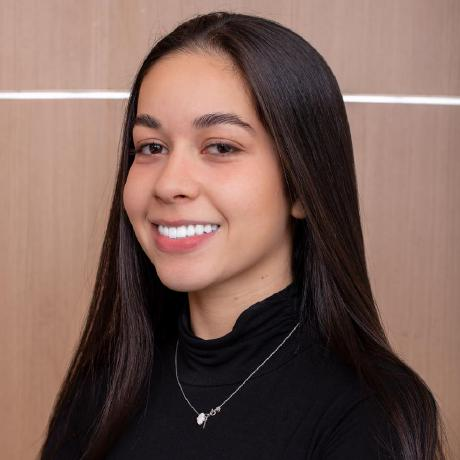
\includegraphics[
                        width=4.20cm,
                        height=4.20cm,
                        keepaspectratio
                    ]{profile.jpg}%
                }
            }
            {
                \fcolorbox{line}{soft}{
                    \parbox[c][4.20cm][c]{4.20cm}{
                        \centering

                        \color{muted}

                        \Large
                        \faUser

                        \par\vspace{0.10cm}

                        \scriptsize
                        profile.jpg
                    }
                }
            }

        \end{minipage}

        \end{tabularx}
    }
    {
        \begin{tabularx}{\linewidth}{
            @{}
            >{\raggedright\arraybackslash}X
            >{\raggedright\arraybackslash}p{6.2cm}
            @{}
        }

        \begin{minipage}[c]{\linewidth}

            \HeaderName{#1}{#2}

        \end{minipage}

        &

        \begin{minipage}[c]{\linewidth}

            \HeaderContacts{#3}{#5}

        \end{minipage}

        \end{tabularx}
    }

    \vspace{0.10cm}

    {\color{primary}
    \rule{\linewidth}{1.15pt}}

    \vspace{0.10cm}
}

% =========================================================
% COMPANY DESCRIPTOR (one line of context under a role)
% =========================================================
\newcommand{\roleinfo}[1]{
    {\small\itshape\color{muted}#1}

    \vspace{-0.03cm}
}

% =========================================================
% =========================================================
% ENGLISH VERSION
% =========================================================
% =========================================================

\newcommand{\EnglishCV}{

% =========================================================
% HEADER
% =========================================================
\CVHeader
{MOBILE SOFTWARE ENGINEER \;|\; FLUTTER DEVELOPER}
{Flutter \;•\; Dart \;•\; Android \& iOS \;•\; 4+ years in production}
{\LocationEN}
{nophoto}
{\WorkModeEN}

% =========================================================
% SUMMARY
% =========================================================
\cvsection{\faUser}{Professional Summary}

{\small
\justifying
Mobile Software Engineer specialized in \textbf{Flutter and Dart}, with 4+
years shipping production apps for Android and iOS and a B.Sc. in Systems
Engineering from UFMG. At \textbf{R10 Score} (1M+ Google Play downloads),
built real-time, high-traffic features end to end, such as the 2026 World Cup
experience and the live bet wall. At Prime Results, turned a white-label app
for 8 client companies into one flavor-based codebase. Strong in
Clean Architecture, BLoC/Cubit, real-time data (WebSocket, Protobuf) and testing;
also delivers with React, NestJS, Java and Spring.
}

% =========================================================
% CORE SKILLS
% =========================================================
\cvsection{\faCode}{Core Technical Skills}

\skillline
{Mobile}
{Flutter, Dart, Android, iOS, Kotlin, Swift, platform channels, flavors /
white-label, adaptive tablet UI, In-App Purchases, React Native}

\skillline
{State \& Architecture}
{BLoC, Cubit, Freezed, GoRouter, Clean Architecture, SOLID, dependency
injection, modular monorepo}

\skillline
{APIs \& Real-Time}
{REST APIs, JSON, Protobuf, WebSocket, Swagger / OpenAPI}

\skillline
{Firebase \& Data}
{Firebase, Crashlytics, Analytics, Realtime Database, feature flags, SQL,
PostgreSQL}

\skillline
{Web \& Backend}
{React, TypeScript, NestJS, Prisma, Java, Spring}

\skillline
{Quality \& Delivery}
{Unit, Widget \& Integration Testing (bloc\_test, mocktail), Code Review, CI/CD, GitHub
Actions, Codemagic, Git, Azure DevOps, Figma, Scrum, AI-assisted development
(Claude Code)}

\skillline
{Languages}
{Portuguese (native), English (professional working proficiency, B2 · TOEFL)}

% =========================================================
% EXPERIENCE
% =========================================================
\cvsection{\faBriefcase}{Professional Experience}

\experience
{Full Stack Developer | Mobile (Flutter)}
{OTG Ventures \;·\; R10 Score}
{Jun 2025 -- Sep 2026}
{
\roleinfo{Live football scores and statistics app \;·\; 1M+ Google
Play downloads \;·\; 11-package Flutter
monorepo}

\begin{itemize}

    \item
    Delivered the \textbf{2026 World Cup experience} (bracket, group tables,
    Favorite Team vote, match guesses and CMS-driven content) in time for the
    tournament's fixed start, joined by
    \textbf{22\% of all accounts}.

    \item
    Main mobile developer on \textbf{Notified Bet}: a live bet wall with
    drag-and-drop ordering saved on the backend (optimistic updates with
    rollback) and live status over \textbf{WebSocket}.

    \item
    \textbf{Unblocked Google Play publishing} after the 2026 target-API
    deadline (targetSdk 36, Play Billing Library 8.0.0), protecting In-App
    Purchase subscription revenue.

    \item
    Brought the test suite back to green, fixing two production bugs along the
    way, and tracked down an intermittent freeze in match statistics; one of
    the team's most active contributors, with \textbf{500+ merged PRs} and
    570+ code reviews.

    \item
    Built on \textbf{WebSocket (Protobuf and JSON) and REST}, with
    \textbf{Firebase} feature flags and Crashlytics; also contributed full stack
    to \textbf{OTG Partners}, the group's affiliate-commission platform
    (\textbf{React, NestJS}, Prisma, PostgreSQL).
\end{itemize}
}

\experience
{Mobile Developer}
{Prime Results}
{May 2022 -- May 2025}
{
\roleinfo{Intern from May 2022, Mobile Developer from Feb 2023 \;·\; white-label app for the
field and point-of-sale teams of 8 client companies \;·\; Android \& iOS}

\begin{itemize}

    \item
    Consolidated a \textbf{white-label app for 8 client companies}, kept on
    separate cherry-picked branches, into \textbf{one codebase with Flutter
    flavors}, so every fix ships to all clients from a single main branch.

    \item
    Adjusted and improved \textbf{phone and tablet layouts} across the app,
    used by field and point-of-sale teams.

    \item
    Delivered features end to end, from \textbf{Figma} to \textbf{REST API}
    integration and releases on \textbf{Google Play and the App Store}, and contributed to \textbf{Java and Spring}
    services and \textbf{React} web projects.
\end{itemize}
}

\experience
{Mobile Developer -- Freelance}
{Upbeat Studio \;·\; Drum Coach app -- Germany (remote)}
{Mar 2025 -- Apr 2025}
{
\begin{itemize}

    \item
    Built an interactive \textbf{Flutter and Dart} app for learning and
    practicing drums, working remotely and autonomously with an international
    team in English.
\end{itemize}
}

\experience
{Programming Instructor (Volunteer)}
{Garotas Aplicadas Project -- AVEC | Centro Universitário Una}
{Jan 2025 -- Aug 2026}
{
\begin{itemize}

    \item
    Taught theory and hands-on programming classes to public
    high-school girls in Belo Horizonte, in a social initiative to
    widen female participation in technology.
\end{itemize}
}

\experience
{Business Analyst \& Front-End Developer}
{iJunior}
{Mar 2022 -- May 2022}
{
\begin{itemize}

    \item
    Gathered requirements with clients and the sales team and built custom
    apps and websites with \textbf{React Native} for organizations across
    different sectors, using \textbf{Scrum and Kanban}.
\end{itemize}
}

\experience
{Systems Analyst}
{Interact Place}
{Oct 2021 -- Jan 2022}
{
\begin{itemize}

    \item
    Helped build an interactive mobile exhibition guide for
    \textbf{Palácio das Artes}, one of Belo Horizonte's major cultural
    institutions, where QR codes connect visitors to artwork information.
\end{itemize}
}

% =========================================================
% EDUCATION
% =========================================================
\cvsection{\faGraduationCap}{Education \& Certifications}

\education
{Bachelor's Degree in Systems Engineering}
{Federal University of Minas Gerais -- UFMG}
{2020 -- 2026}
{}

\skillline
{Certifications}
{TOEFL (English, B2) \;·\; CCAA English course (2008 -- 2019) \;·\; Google
Play Academy -- Store Listing Certificate}

}


% =========================================================
% =========================================================
% PORTUGUESE VERSION
% =========================================================
% =========================================================

\newcommand{\PortugueseCV}{

% =========================================================
% HEADER
% =========================================================
\CVHeader
{ENGENHEIRA DE SOFTWARE MOBILE \;|\; DESENVOLVEDORA FLUTTER}
{Flutter \;•\; Dart \;•\; Android e iOS \;•\; 4+ anos em produção}
{\LocationPT}
{photo}
{\WorkModePT}

% =========================================================
% SUMMARY
% =========================================================
\cvsection{\faUser}{Resumo Profissional}

{\small
\justifying
Engenheira de Software Mobile especializada em \textbf{Flutter e Dart}, com
mais de 4 anos entregando apps em produção para Android e iOS, formada em
Engenharia de Sistemas pela UFMG. No \textbf{R10 Score} (mais de 1 milhão de
downloads no Google Play), desenvolvi de ponta a ponta funcionalidades em tempo
real e de alto tráfego, como a experiência da Copa do Mundo 2026 e o mural de
apostas ao vivo. Na Prime Results, transformei um app white-label de 8 empresas
clientes em um único código com flavors. Forte em Clean Architecture,
BLoC/Cubit, dados em tempo real (WebSocket, Protobuf) e testes; também atuo com
React, NestJS, Java e Spring.
}

% =========================================================
% CORE SKILLS
% =========================================================
\cvsection{\faCode}{Competências Técnicas}

\skillline
{Mobile}
{Flutter, Dart, Android, iOS, Kotlin, Swift, platform channels, flavors /
white-label, UI adaptativa para tablet, compras in-app, React Native}

\skillline
{Estado \& Arquitetura}
{BLoC, Cubit, Freezed, GoRouter, Clean Architecture, SOLID, injeção de
dependência, monorepo modular}

\skillline
{APIs \& Tempo Real}
{APIs REST, JSON, Protobuf, WebSocket, Swagger / OpenAPI}

\skillline
{Firebase \& Dados}
{Firebase, Crashlytics, Analytics, Realtime Database, feature flags, SQL,
PostgreSQL}

\skillline
{Web \& Backend}
{React, TypeScript, NestJS, Prisma, Java, Spring}

\skillline
{Qualidade \& Entrega}
{Testes Unitários, de Widget e de Integração (bloc\_test, mocktail), Code Review, CI/CD,
GitHub Actions, Codemagic, Git, Azure DevOps, Figma, Scrum, desenvolvimento
assistido por IA (Claude Code)}

\skillline
{Idiomas}
{Português (nativo), Inglês (proficiência profissional, B2 · TOEFL)}

% =========================================================
% EXPERIENCE
% =========================================================
\cvsection{\faBriefcase}{Experiência Profissional}

\experience
{Desenvolvedora Full Stack | Mobile (Flutter)}
{OTG Ventures \;·\; R10 Score}
{Jun 2025 -- Set 2026}
{
\roleinfo{App de placares e estatísticas de futebol ao vivo \;·\;
mais de 1 milhão de downloads no Google Play \;·\; monorepo Flutter com 11 pacotes}

\begin{itemize}

    \item
    Entreguei a \textbf{experiência da Copa do Mundo 2026} (chaveamento,
    tabela de grupos, votação do Time do Coração, palpites e conteúdo via CMS)
    a tempo do início do torneio, com adesão de
    \textbf{22\% de todas as contas}.

    \item
    Principal desenvolvedora mobile da \textbf{Aposta Notificada}: mural de apostas ao vivo
    com reordenação por drag-and-drop salva no backend (atualização otimista
    com rollback) e status em tempo real via \textbf{WebSocket}.

    \item
    \textbf{Desbloqueei a publicação no Google Play} após o prazo de target
    API de 2026 (targetSdk 36, Play Billing Library 8.0.0), protegendo a
    receita das assinaturas (compras in-app).

    \item
    Recuperei a suíte de testes, corrigindo dois bugs de produção no caminho,
    e rastreei um travamento intermitente nas estatísticas das partidas; estou
    entre as pessoas mais ativas do time, com \textbf{mais de 500 PRs}
    mergeados e mais de 570 code reviews.

    \item
    Desenvolvi sobre \textbf{WebSocket (Protobuf e JSON) e REST}, com
    feature flags no \textbf{Firebase} e Crashlytics; atuei também full stack
    no \textbf{OTG Partners}, plataforma de comissões de afiliados do grupo
    (\textbf{React, NestJS}, Prisma, PostgreSQL).
\end{itemize}
}

\experience
{Desenvolvedora Mobile}
{Prime Results}
{Mai 2022 -- Mai 2025}
{
\roleinfo{Estagiária desde mai 2022, Desenvolvedora Mobile desde fev 2023 \;·\; app
white-label para equipes de campo e de ponto de venda de 8 empresas clientes}

\begin{itemize}

    \item
    Consolidei um \textbf{app white-label de 8 empresas clientes}, mantido em
    branches separadas sincronizadas por cherry-pick, em \textbf{um único
    código com flavors do Flutter}, para que cada correção chegue a todos os
    clientes a partir de uma única branch principal.

    \item
    Ajustei e melhorei \textbf{layouts para celular e tablet} em todo o app,
    usado por equipes de campo e de ponto de venda.

    \item
    Entreguei funcionalidades de ponta a ponta, do \textbf{Figma} à
    integração com \textbf{APIs REST} e à publicação no \textbf{Google Play e na App Store}, e contribuí em serviços
    \textbf{Java e Spring} e em projetos web com \textbf{React}.
\end{itemize}
}

\experience
{Desenvolvedora Mobile -- Freelancer}
{Upbeat Studio \;·\; app Drum Coach -- Alemanha (remoto)}
{Mar 2025 -- Abr 2025}
{
\begin{itemize}

    \item
    Desenvolvi um app interativo em \textbf{Flutter e Dart} para aprender e
    praticar bateria, em trabalho remoto e autônomo com uma equipe
    internacional, em inglês.
\end{itemize}
}

\experience
{Instrutora de Programação (Voluntária)}
{Projeto Garotas Aplicadas -- AVEC | Centro Universitário Una}
{Jan 2025 -- Ago 2026}
{
\begin{itemize}

    \item
    Dei aulas teóricas e práticas de programação para estudantes do ensino
    médio da rede pública de Belo Horizonte, em uma iniciativa social para
    ampliar a participação feminina na tecnologia.
\end{itemize}
}

\experience
{Analista de Negócios \& Desenvolvedora Front-End}
{iJunior}
{Mar 2022 -- Mai 2022}
{
\begin{itemize}

    \item
    Levantei requisitos com clientes e com a equipe comercial e desenvolvi
    aplicações e websites personalizados com \textbf{React Native} para
    organizações de diferentes segmentos, com \textbf{Scrum e Kanban}.
\end{itemize}
}

\experience
{Analista de Sistemas}
{Interact Place}
{Out 2021 -- Jan 2022}
{
\begin{itemize}

    \item
    Participei do desenvolvimento de um guia mobile interativo de exposições
    para o \textbf{Palácio das Artes}, uma das principais instituições
    culturais de Belo Horizonte, em que QR Codes conectam os visitantes a
    informações sobre as obras.
\end{itemize}
}

% =========================================================
% EDUCATION
% =========================================================
\cvsection{\faGraduationCap}{Formação \& Certificações}

\education
{Bacharelado em Engenharia de Sistemas}
{Universidade Federal de Minas Gerais -- UFMG}
{2020 -- 2026}
{}

\skillline
{Certificações}
{TOEFL (inglês, B2) \;·\; Curso de inglês CCAA (2008 -- 2019) \;·\; Google
Play Academy -- Store Listing Certificate}

}

% =========================================================
% LANGUAGE-SPECIFIC PDF METADATA
% =========================================================
\newcommand{\MetadataEN}{
    \hypersetup{
        pdftitle={Beatriz Vocurca Frade - Mobile Software Engineer - Flutter Developer},
        pdfsubject={Mobile Software Engineering, Flutter and Software Development Resume},
        pdflang={en-US}
    }
}

\newcommand{\MetadataPT}{
    \hypersetup{
        pdftitle={Beatriz Vocurca Frade - Engenheira de Software Mobile - Desenvolvedora Flutter},
        pdfsubject={Currículo de Engenharia de Software Mobile, Flutter e Desenvolvimento de Software},
        pdflang={pt-BR}
    }
}

\ifthenelse{\equal{\CVLang}{pt}}
{\MetadataPT}
{\MetadataEN}


% =========================================================
% DOCUMENT
% =========================================================
\begin{document}

\ifthenelse{\equal{\CVLang}{en}}
{
    \EnglishCV
}
{
    \ifthenelse{\equal{\CVLang}{pt}}
    {
        \PortugueseCV
    }
    {
        % Bilingual: English first, Portuguese after a page break
        \EnglishCV

        \newpage

        \PortugueseCV
    }
}

\end{document}
"
% =========================================================

\providecommand{\CVLang}{both}

% =========================================================
% PACKAGES
% =========================================================
\usepackage[
    top=0.85cm,
    bottom=0.85cm,
    left=1.15cm,
    right=1.15cm
]{geometry}

\usepackage[T1]{fontenc}
\usepackage[utf8]{inputenc}
% Source Sans Pro ships with TeX Live / Overleaf (lmodern is not installed
% on every machine, which broke the build).
\usepackage[default,lining]{sourcesanspro}
\usepackage{microtype}
\usepackage{xcolor}
\usepackage{graphicx}
\usepackage{fontawesome5}
\usepackage{enumitem}
\usepackage{tabularx}
\usepackage{array}
\usepackage{hyperref}
\usepackage{ragged2e}
\usepackage{needspace}
\usepackage{ifthen}

% Improves PDF text extraction for ATS / AI systems
\input{glyphtounicode}
\pdfgentounicode=1

% ATS: icons are decorative. Map every icon glyph to a plain space so text
% extractors never emit stray characters next to contact details or headings.
\pdfglyphtounicode{map-marker}{0020}
\pdfglyphtounicode{map-marker-alt}{0020}
\pdfglyphtounicode{laptop}{0020}
\pdfglyphtounicode{phone}{0020}
\pdfglyphtounicode{envelope}{0020}
\pdfglyphtounicode{linkedin}{0020}
\pdfglyphtounicode{github}{0020}
\pdfglyphtounicode{user}{0020}
\pdfglyphtounicode{code}{0020}
\pdfglyphtounicode{briefcase}{0020}
\pdfglyphtounicode{graduation-cap}{0020}
\pdfglyphtounicode{certificate}{0020}

% ATS: write real space characters into the PDF text layer, so parsers never
% glue words at font changes ("inFlutter"), which breaks keyword matching.
\pdfinterwordspaceon

% =========================================================
% GLOBAL CONFIGURATION
% =========================================================
\pagestyle{empty}

\setlength{\parindent}{0pt}
\setlength{\parskip}{0pt}

\renewcommand{\familydefault}{\sfdefault}

% \justifying (ragged2e) would otherwise indent every new paragraph
\setlength{\JustifyingParindent}{0pt}

\clubpenalty=10000
\widowpenalty=10000

% ATS: never hyphenate, so keywords are never split across lines.
\hyphenpenalty=10000
\exhyphenpenalty=10000
\emergencystretch=2em

% =========================================================
% COLORS
% =========================================================
\definecolor{primary}{HTML}{223846}
\definecolor{accent}{HTML}{3F6678}
\definecolor{muted}{HTML}{66747D}
\definecolor{text}{HTML}{20252A}
\definecolor{line}{HTML}{CDD7DC}
\definecolor{soft}{HTML}{F3F6F7}
\definecolor{white}{HTML}{FFFFFF}

% =========================================================
% PERSONAL INFORMATION
% =========================================================
\newcommand{\FullName}{Beatriz Vocurca Frade}

\newcommand{\Email}
{beatrizvocurcafrade@gmail.com}

\newcommand{\LinkedInURL}
{https://www.linkedin.com/in/beatriz-mobile/}

\newcommand{\LinkedInText}
{linkedin.com/in/beatriz-mobile}

\newcommand{\GitHubURL}
{https://github.com/BeatrizVocurcaFrade}

\newcommand{\GitHubText}
{github.com/BeatrizVocurcaFrade}

\newcommand{\LocationEN}
{Belo Horizonte, Minas Gerais, Brazil}

\newcommand{\LocationPT}
{Belo Horizonte, Minas Gerais, Brasil}

\newcommand{\WorkModeEN}
{Remote (UTC-3) · available immediately}

\newcommand{\WorkModePT}
{Remoto ou híbrido em BH · disponibilidade imediata}

% =========================================================
% PDF / LINKS
% =========================================================
\hypersetup{
    colorlinks=true,
    urlcolor=accent,
    linkcolor=accent,
    pdfauthor={Beatriz Vocurca Frade},
    pdfkeywords={
        Flutter,
        Dart,
        Flutter Developer,
        Mobile Developer,
        Mobile Software Engineer,
        Software Engineer,
        Mobile Engineer,
        Android,
        iOS,
        BLoC,
        Cubit,
        Freezed,
        GoRouter,
        Flavors,
        White-label,
        Platform Channels,
        Kotlin,
        Swift,
        In-App Purchases,
        Firebase,
        Crashlytics,
        Analytics,
        Firebase Realtime Database,
        Feature Flags,
        REST API,
        REST APIs,
        API Integration,
        Protobuf,
        WebSocket,
        JSON,
        React,
        React Native,
        TypeScript,
        NestJS,
        Prisma,
        PostgreSQL,
        Java,
        Spring,
        SQL,
        Clean Architecture,
        Clean Code,
        SOLID,
        Design Patterns,
        Git,
        GitHub,
        GitHub Actions,
        Codemagic,
        Azure DevOps,
        CI/CD,
        Figma,
        Swagger,
        Automated Testing,
        Unit Testing,
        Widget Testing,
        Code Review,
        Refactoring,
        Debugging,
        Performance,
        Agile,
        Scrum,
        Kanban,
        Football,
        Sports Data,
        Live Sports,
        Football Statistics
    }
}

\urlstyle{same}

% =========================================================
% LIST CONFIGURATION
% =========================================================
\setlist[itemize]{
    leftmargin=0.43cm,
    itemsep=0.035cm,
    topsep=0.055cm,
    parsep=0pt,
    partopsep=0pt
}

% =========================================================
% SECTION
% =========================================================
\newcommand{\cvsection}[2]{

    \needspace{4\baselineskip}

    \vspace{0.18cm}

    {\large
    \bfseries
    \color{primary}
    #1
    \hspace{0.10cm}
    #2}

    \vspace{0.025cm}

    {\color{line}
    \rule{\linewidth}{0.65pt}}

    \vspace{0.07cm}
}

% =========================================================
% EXPERIENCE
% =========================================================
\newcommand{\experience}[4]{

    \needspace{5\baselineskip}

    \begin{tabularx}{\linewidth}{
        @{}
        >{\raggedright\arraybackslash}X
        >{\raggedleft\arraybackslash}p{3.25cm}
        @{}
    }

    {\bfseries\color{text}#1}
    &
    {\small\bfseries\color{accent}#3}
    \\[-0.01cm]
    {\small
    \bfseries
    \color{muted}
    #2}
    &
    \end{tabularx}

    \vspace{-0.09cm}

    {\small
    \color{text}
    #4
    }

    \vspace{0.07cm}
}

% =========================================================
% EDUCATION
% =========================================================
\newcommand{\education}[4]{

    \needspace{3\baselineskip}

    \begin{tabularx}{\linewidth}{
        @{}
        >{\raggedright\arraybackslash}X
        >{\raggedleft\arraybackslash}p{3.1cm}
        @{}
    }

    {\bfseries\color{text}#1}
    &
    {\small\bfseries\color{accent}#3}
    \\[-0.01cm]
    {\small\color{muted}#2}
    &
    \end{tabularx}

    \ifthenelse{\equal{#4}{}}
    {}
    {
        {\small\color{text}#4}
    }

    \vspace{0.09cm}
}

% =========================================================
% SKILL LINE
% =========================================================
\newcommand{\skillline}[2]{
    {\small
    \textbf{\color{primary}#1:}
    \color{text}
    #2
    }

    \vspace{0.045cm}
}

% =========================================================
% HEADER
%
% #1 title, #2 keyword line, #3 location, #4 photo | nophoto, #5 work mode
% (the English version omits the photo, as most international
% recruiters expect; the Portuguese version keeps it)
% =========================================================
\newcommand{\HeaderName}[2]{
    {\fontsize{24}{27}\selectfont
    \bfseries
    \color{primary}
    \FullName}

    \vspace{0.045cm}

    {\normalsize
    \bfseries
    \color{accent}
    #1}

    \vspace{0.055cm}

    {\small
    \color{muted}
    #2}
}

\newcommand{\HeaderContacts}[2]{
    {\small
    \color{text}

    \faMapMarker
    \hspace{0.045cm}
    #1

    \par\vspace{0.08cm}

    \faLaptop
    \hspace{0.045cm}
    #2

    \par\vspace{0.08cm}

    \faEnvelope
    \hspace{0.045cm}
    \href{mailto:\Email}{\Email}

    \par\vspace{0.08cm}

    \faLinkedin
    \hspace{0.045cm}
    \href{\LinkedInURL}{\LinkedInText}

    \par\vspace{0.08cm}

    \faGithub
    \hspace{0.045cm}
    \href{\GitHubURL}{\GitHubText}

    }
}

\newcommand{\CVHeader}[5]{

    \noindent
    \ifthenelse{\equal{#4}{photo}}
    {
        \begin{tabularx}{\linewidth}{
            @{}
            >{\raggedright\arraybackslash}X
            >{\centering\arraybackslash}p{4.45cm}
            @{}
        }

        \begin{minipage}[c]{\linewidth}

            \HeaderName{#1}{#2}

            \vspace{0.15cm}

            \HeaderContacts{#3}{#5}

        \end{minipage}

        &

        % PROFILE PHOTO (profile.jpg next to this file)
        \begin{minipage}[c]{4.35cm}

            \centering

            \IfFileExists{profile.jpg}
            {
                \fcolorbox{line}{white}{%
                    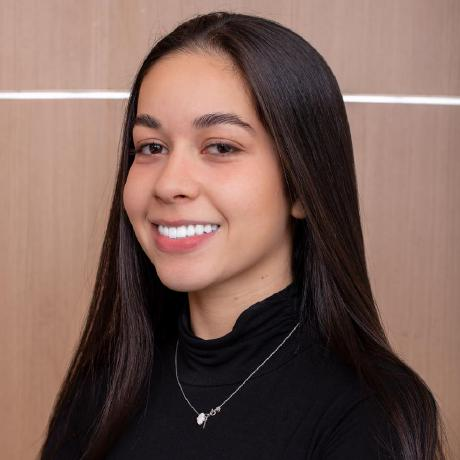
\includegraphics[
                        width=4.20cm,
                        height=4.20cm,
                        keepaspectratio
                    ]{profile.jpg}%
                }
            }
            {
                \fcolorbox{line}{soft}{
                    \parbox[c][4.20cm][c]{4.20cm}{
                        \centering

                        \color{muted}

                        \Large
                        \faUser

                        \par\vspace{0.10cm}

                        \scriptsize
                        profile.jpg
                    }
                }
            }

        \end{minipage}

        \end{tabularx}
    }
    {
        \begin{tabularx}{\linewidth}{
            @{}
            >{\raggedright\arraybackslash}X
            >{\raggedright\arraybackslash}p{6.2cm}
            @{}
        }

        \begin{minipage}[c]{\linewidth}

            \HeaderName{#1}{#2}

        \end{minipage}

        &

        \begin{minipage}[c]{\linewidth}

            \HeaderContacts{#3}{#5}

        \end{minipage}

        \end{tabularx}
    }

    \vspace{0.10cm}

    {\color{primary}
    \rule{\linewidth}{1.15pt}}

    \vspace{0.10cm}
}

% =========================================================
% COMPANY DESCRIPTOR (one line of context under a role)
% =========================================================
\newcommand{\roleinfo}[1]{
    {\small\itshape\color{muted}#1}

    \vspace{-0.03cm}
}

% =========================================================
% =========================================================
% ENGLISH VERSION
% =========================================================
% =========================================================

\newcommand{\EnglishCV}{

% =========================================================
% HEADER
% =========================================================
\CVHeader
{MOBILE SOFTWARE ENGINEER \;|\; FLUTTER DEVELOPER}
{Flutter \;•\; Dart \;•\; Android \& iOS \;•\; 4+ years in production}
{\LocationEN}
{nophoto}
{\WorkModeEN}

% =========================================================
% SUMMARY
% =========================================================
\cvsection{\faUser}{Professional Summary}

{\small
\justifying
Mobile Software Engineer specialized in \textbf{Flutter and Dart}, with 4+
years shipping production apps for Android and iOS and a B.Sc. in Systems
Engineering from UFMG. At \textbf{R10 Score} (1M+ Google Play downloads),
built real-time, high-traffic features end to end, such as the 2026 World Cup
experience and the live bet wall. At Prime Results, turned a white-label app
for 8 client companies into one flavor-based codebase. Strong in
Clean Architecture, BLoC/Cubit, real-time data (WebSocket, Protobuf) and testing;
also delivers with React, NestJS, Java and Spring.
}

% =========================================================
% CORE SKILLS
% =========================================================
\cvsection{\faCode}{Core Technical Skills}

\skillline
{Mobile}
{Flutter, Dart, Android, iOS, Kotlin, Swift, platform channels, flavors /
white-label, adaptive tablet UI, In-App Purchases, React Native}

\skillline
{State \& Architecture}
{BLoC, Cubit, Freezed, GoRouter, Clean Architecture, SOLID, dependency
injection, modular monorepo}

\skillline
{APIs \& Real-Time}
{REST APIs, JSON, Protobuf, WebSocket, Swagger / OpenAPI}

\skillline
{Firebase \& Data}
{Firebase, Crashlytics, Analytics, Realtime Database, feature flags, SQL,
PostgreSQL}

\skillline
{Web \& Backend}
{React, TypeScript, NestJS, Prisma, Java, Spring}

\skillline
{Quality \& Delivery}
{Unit, Widget \& Integration Testing (bloc\_test, mocktail), Code Review, CI/CD, GitHub
Actions, Codemagic, Git, Azure DevOps, Figma, Scrum, AI-assisted development
(Claude Code)}

\skillline
{Languages}
{Portuguese (native), English (professional working proficiency, B2 · TOEFL)}

% =========================================================
% EXPERIENCE
% =========================================================
\cvsection{\faBriefcase}{Professional Experience}

\experience
{Full Stack Developer | Mobile (Flutter)}
{OTG Ventures \;·\; R10 Score}
{Jun 2025 -- Sep 2026}
{
\roleinfo{Live football scores and statistics app \;·\; 1M+ Google
Play downloads \;·\; 11-package Flutter
monorepo}

\begin{itemize}

    \item
    Delivered the \textbf{2026 World Cup experience} (bracket, group tables,
    Favorite Team vote, match guesses and CMS-driven content) in time for the
    tournament's fixed start, joined by
    \textbf{22\% of all accounts}.

    \item
    Main mobile developer on \textbf{Notified Bet}: a live bet wall with
    drag-and-drop ordering saved on the backend (optimistic updates with
    rollback) and live status over \textbf{WebSocket}.

    \item
    \textbf{Unblocked Google Play publishing} after the 2026 target-API
    deadline (targetSdk 36, Play Billing Library 8.0.0), protecting In-App
    Purchase subscription revenue.

    \item
    Brought the test suite back to green, fixing two production bugs along the
    way, and tracked down an intermittent freeze in match statistics; one of
    the team's most active contributors, with \textbf{500+ merged PRs} and
    570+ code reviews.

    \item
    Built on \textbf{WebSocket (Protobuf and JSON) and REST}, with
    \textbf{Firebase} feature flags and Crashlytics; also contributed full stack
    to \textbf{OTG Partners}, the group's affiliate-commission platform
    (\textbf{React, NestJS}, Prisma, PostgreSQL).
\end{itemize}
}

\experience
{Mobile Developer}
{Prime Results}
{May 2022 -- May 2025}
{
\roleinfo{Intern from May 2022, Mobile Developer from Feb 2023 \;·\; white-label app for the
field and point-of-sale teams of 8 client companies \;·\; Android \& iOS}

\begin{itemize}

    \item
    Consolidated a \textbf{white-label app for 8 client companies}, kept on
    separate cherry-picked branches, into \textbf{one codebase with Flutter
    flavors}, so every fix ships to all clients from a single main branch.

    \item
    Adjusted and improved \textbf{phone and tablet layouts} across the app,
    used by field and point-of-sale teams.

    \item
    Delivered features end to end, from \textbf{Figma} to \textbf{REST API}
    integration and releases on \textbf{Google Play and the App Store}, and contributed to \textbf{Java and Spring}
    services and \textbf{React} web projects.
\end{itemize}
}

\experience
{Mobile Developer -- Freelance}
{Upbeat Studio \;·\; Drum Coach app -- Germany (remote)}
{Mar 2025 -- Apr 2025}
{
\begin{itemize}

    \item
    Built an interactive \textbf{Flutter and Dart} app for learning and
    practicing drums, working remotely and autonomously with an international
    team in English.
\end{itemize}
}

\experience
{Programming Instructor (Volunteer)}
{Garotas Aplicadas Project -- AVEC | Centro Universitário Una}
{Jan 2025 -- Aug 2026}
{
\begin{itemize}

    \item
    Taught theory and hands-on programming classes to public
    high-school girls in Belo Horizonte, in a social initiative to
    widen female participation in technology.
\end{itemize}
}

\experience
{Business Analyst \& Front-End Developer}
{iJunior}
{Mar 2022 -- May 2022}
{
\begin{itemize}

    \item
    Gathered requirements with clients and the sales team and built custom
    apps and websites with \textbf{React Native} for organizations across
    different sectors, using \textbf{Scrum and Kanban}.
\end{itemize}
}

\experience
{Systems Analyst}
{Interact Place}
{Oct 2021 -- Jan 2022}
{
\begin{itemize}

    \item
    Helped build an interactive mobile exhibition guide for
    \textbf{Palácio das Artes}, one of Belo Horizonte's major cultural
    institutions, where QR codes connect visitors to artwork information.
\end{itemize}
}

% =========================================================
% EDUCATION
% =========================================================
\cvsection{\faGraduationCap}{Education \& Certifications}

\education
{Bachelor's Degree in Systems Engineering}
{Federal University of Minas Gerais -- UFMG}
{2020 -- 2026}
{}

\skillline
{Certifications}
{TOEFL (English, B2) \;·\; CCAA English course (2008 -- 2019) \;·\; Google
Play Academy -- Store Listing Certificate}

}


% =========================================================
% =========================================================
% PORTUGUESE VERSION
% =========================================================
% =========================================================

\newcommand{\PortugueseCV}{

% =========================================================
% HEADER
% =========================================================
\CVHeader
{ENGENHEIRA DE SOFTWARE MOBILE \;|\; DESENVOLVEDORA FLUTTER}
{Flutter \;•\; Dart \;•\; Android e iOS \;•\; 4+ anos em produção}
{\LocationPT}
{photo}
{\WorkModePT}

% =========================================================
% SUMMARY
% =========================================================
\cvsection{\faUser}{Resumo Profissional}

{\small
\justifying
Engenheira de Software Mobile especializada em \textbf{Flutter e Dart}, com
mais de 4 anos entregando apps em produção para Android e iOS, formada em
Engenharia de Sistemas pela UFMG. No \textbf{R10 Score} (mais de 1 milhão de
downloads no Google Play), desenvolvi de ponta a ponta funcionalidades em tempo
real e de alto tráfego, como a experiência da Copa do Mundo 2026 e o mural de
apostas ao vivo. Na Prime Results, transformei um app white-label de 8 empresas
clientes em um único código com flavors. Forte em Clean Architecture,
BLoC/Cubit, dados em tempo real (WebSocket, Protobuf) e testes; também atuo com
React, NestJS, Java e Spring.
}

% =========================================================
% CORE SKILLS
% =========================================================
\cvsection{\faCode}{Competências Técnicas}

\skillline
{Mobile}
{Flutter, Dart, Android, iOS, Kotlin, Swift, platform channels, flavors /
white-label, UI adaptativa para tablet, compras in-app, React Native}

\skillline
{Estado \& Arquitetura}
{BLoC, Cubit, Freezed, GoRouter, Clean Architecture, SOLID, injeção de
dependência, monorepo modular}

\skillline
{APIs \& Tempo Real}
{APIs REST, JSON, Protobuf, WebSocket, Swagger / OpenAPI}

\skillline
{Firebase \& Dados}
{Firebase, Crashlytics, Analytics, Realtime Database, feature flags, SQL,
PostgreSQL}

\skillline
{Web \& Backend}
{React, TypeScript, NestJS, Prisma, Java, Spring}

\skillline
{Qualidade \& Entrega}
{Testes Unitários, de Widget e de Integração (bloc\_test, mocktail), Code Review, CI/CD,
GitHub Actions, Codemagic, Git, Azure DevOps, Figma, Scrum, desenvolvimento
assistido por IA (Claude Code)}

\skillline
{Idiomas}
{Português (nativo), Inglês (proficiência profissional, B2 · TOEFL)}

% =========================================================
% EXPERIENCE
% =========================================================
\cvsection{\faBriefcase}{Experiência Profissional}

\experience
{Desenvolvedora Full Stack | Mobile (Flutter)}
{OTG Ventures \;·\; R10 Score}
{Jun 2025 -- Set 2026}
{
\roleinfo{App de placares e estatísticas de futebol ao vivo \;·\;
mais de 1 milhão de downloads no Google Play \;·\; monorepo Flutter com 11 pacotes}

\begin{itemize}

    \item
    Entreguei a \textbf{experiência da Copa do Mundo 2026} (chaveamento,
    tabela de grupos, votação do Time do Coração, palpites e conteúdo via CMS)
    a tempo do início do torneio, com adesão de
    \textbf{22\% de todas as contas}.

    \item
    Principal desenvolvedora mobile da \textbf{Aposta Notificada}: mural de apostas ao vivo
    com reordenação por drag-and-drop salva no backend (atualização otimista
    com rollback) e status em tempo real via \textbf{WebSocket}.

    \item
    \textbf{Desbloqueei a publicação no Google Play} após o prazo de target
    API de 2026 (targetSdk 36, Play Billing Library 8.0.0), protegendo a
    receita das assinaturas (compras in-app).

    \item
    Recuperei a suíte de testes, corrigindo dois bugs de produção no caminho,
    e rastreei um travamento intermitente nas estatísticas das partidas; estou
    entre as pessoas mais ativas do time, com \textbf{mais de 500 PRs}
    mergeados e mais de 570 code reviews.

    \item
    Desenvolvi sobre \textbf{WebSocket (Protobuf e JSON) e REST}, com
    feature flags no \textbf{Firebase} e Crashlytics; atuei também full stack
    no \textbf{OTG Partners}, plataforma de comissões de afiliados do grupo
    (\textbf{React, NestJS}, Prisma, PostgreSQL).
\end{itemize}
}

\experience
{Desenvolvedora Mobile}
{Prime Results}
{Mai 2022 -- Mai 2025}
{
\roleinfo{Estagiária desde mai 2022, Desenvolvedora Mobile desde fev 2023 \;·\; app
white-label para equipes de campo e de ponto de venda de 8 empresas clientes}

\begin{itemize}

    \item
    Consolidei um \textbf{app white-label de 8 empresas clientes}, mantido em
    branches separadas sincronizadas por cherry-pick, em \textbf{um único
    código com flavors do Flutter}, para que cada correção chegue a todos os
    clientes a partir de uma única branch principal.

    \item
    Ajustei e melhorei \textbf{layouts para celular e tablet} em todo o app,
    usado por equipes de campo e de ponto de venda.

    \item
    Entreguei funcionalidades de ponta a ponta, do \textbf{Figma} à
    integração com \textbf{APIs REST} e à publicação no \textbf{Google Play e na App Store}, e contribuí em serviços
    \textbf{Java e Spring} e em projetos web com \textbf{React}.
\end{itemize}
}

\experience
{Desenvolvedora Mobile -- Freelancer}
{Upbeat Studio \;·\; app Drum Coach -- Alemanha (remoto)}
{Mar 2025 -- Abr 2025}
{
\begin{itemize}

    \item
    Desenvolvi um app interativo em \textbf{Flutter e Dart} para aprender e
    praticar bateria, em trabalho remoto e autônomo com uma equipe
    internacional, em inglês.
\end{itemize}
}

\experience
{Instrutora de Programação (Voluntária)}
{Projeto Garotas Aplicadas -- AVEC | Centro Universitário Una}
{Jan 2025 -- Ago 2026}
{
\begin{itemize}

    \item
    Dei aulas teóricas e práticas de programação para estudantes do ensino
    médio da rede pública de Belo Horizonte, em uma iniciativa social para
    ampliar a participação feminina na tecnologia.
\end{itemize}
}

\experience
{Analista de Negócios \& Desenvolvedora Front-End}
{iJunior}
{Mar 2022 -- Mai 2022}
{
\begin{itemize}

    \item
    Levantei requisitos com clientes e com a equipe comercial e desenvolvi
    aplicações e websites personalizados com \textbf{React Native} para
    organizações de diferentes segmentos, com \textbf{Scrum e Kanban}.
\end{itemize}
}

\experience
{Analista de Sistemas}
{Interact Place}
{Out 2021 -- Jan 2022}
{
\begin{itemize}

    \item
    Participei do desenvolvimento de um guia mobile interativo de exposições
    para o \textbf{Palácio das Artes}, uma das principais instituições
    culturais de Belo Horizonte, em que QR Codes conectam os visitantes a
    informações sobre as obras.
\end{itemize}
}

% =========================================================
% EDUCATION
% =========================================================
\cvsection{\faGraduationCap}{Formação \& Certificações}

\education
{Bacharelado em Engenharia de Sistemas}
{Universidade Federal de Minas Gerais -- UFMG}
{2020 -- 2026}
{}

\skillline
{Certificações}
{TOEFL (inglês, B2) \;·\; Curso de inglês CCAA (2008 -- 2019) \;·\; Google
Play Academy -- Store Listing Certificate}

}

% =========================================================
% LANGUAGE-SPECIFIC PDF METADATA
% =========================================================
\newcommand{\MetadataEN}{
    \hypersetup{
        pdftitle={Beatriz Vocurca Frade - Mobile Software Engineer - Flutter Developer},
        pdfsubject={Mobile Software Engineering, Flutter and Software Development Resume},
        pdflang={en-US}
    }
}

\newcommand{\MetadataPT}{
    \hypersetup{
        pdftitle={Beatriz Vocurca Frade - Engenheira de Software Mobile - Desenvolvedora Flutter},
        pdfsubject={Currículo de Engenharia de Software Mobile, Flutter e Desenvolvimento de Software},
        pdflang={pt-BR}
    }
}

\ifthenelse{\equal{\CVLang}{pt}}
{\MetadataPT}
{\MetadataEN}


% =========================================================
% DOCUMENT
% =========================================================
\begin{document}

\ifthenelse{\equal{\CVLang}{en}}
{
    \EnglishCV
}
{
    \ifthenelse{\equal{\CVLang}{pt}}
    {
        \PortugueseCV
    }
    {
        % Bilingual: English first, Portuguese after a page break
        \EnglishCV

        \newpage

        \PortugueseCV
    }
}

\end{document}
"
% =========================================================

\providecommand{\CVLang}{both}

% =========================================================
% PACKAGES
% =========================================================
\usepackage[
    top=0.85cm,
    bottom=0.85cm,
    left=1.15cm,
    right=1.15cm
]{geometry}

\usepackage[T1]{fontenc}
\usepackage[utf8]{inputenc}
% Source Sans Pro ships with TeX Live / Overleaf (lmodern is not installed
% on every machine, which broke the build).
\usepackage[default,lining]{sourcesanspro}
\usepackage{microtype}
\usepackage{xcolor}
\usepackage{graphicx}
\usepackage{fontawesome5}
\usepackage{enumitem}
\usepackage{tabularx}
\usepackage{array}
\usepackage{hyperref}
\usepackage{ragged2e}
\usepackage{needspace}
\usepackage{ifthen}

% Improves PDF text extraction for ATS / AI systems
\input{glyphtounicode}
\pdfgentounicode=1

% ATS: icons are decorative. Map every icon glyph to a plain space so text
% extractors never emit stray characters next to contact details or headings.
\pdfglyphtounicode{map-marker}{0020}
\pdfglyphtounicode{map-marker-alt}{0020}
\pdfglyphtounicode{laptop}{0020}
\pdfglyphtounicode{phone}{0020}
\pdfglyphtounicode{envelope}{0020}
\pdfglyphtounicode{linkedin}{0020}
\pdfglyphtounicode{github}{0020}
\pdfglyphtounicode{user}{0020}
\pdfglyphtounicode{code}{0020}
\pdfglyphtounicode{briefcase}{0020}
\pdfglyphtounicode{graduation-cap}{0020}
\pdfglyphtounicode{certificate}{0020}

% ATS: write real space characters into the PDF text layer, so parsers never
% glue words at font changes ("inFlutter"), which breaks keyword matching.
\pdfinterwordspaceon

% =========================================================
% GLOBAL CONFIGURATION
% =========================================================
\pagestyle{empty}

\setlength{\parindent}{0pt}
\setlength{\parskip}{0pt}

\renewcommand{\familydefault}{\sfdefault}

% \justifying (ragged2e) would otherwise indent every new paragraph
\setlength{\JustifyingParindent}{0pt}

\clubpenalty=10000
\widowpenalty=10000

% ATS: never hyphenate, so keywords are never split across lines.
\hyphenpenalty=10000
\exhyphenpenalty=10000
\emergencystretch=2em

% =========================================================
% COLORS
% =========================================================
\definecolor{primary}{HTML}{223846}
\definecolor{accent}{HTML}{3F6678}
\definecolor{muted}{HTML}{66747D}
\definecolor{text}{HTML}{20252A}
\definecolor{line}{HTML}{CDD7DC}
\definecolor{soft}{HTML}{F3F6F7}
\definecolor{white}{HTML}{FFFFFF}

% =========================================================
% PERSONAL INFORMATION
% =========================================================
\newcommand{\FullName}{Beatriz Vocurca Frade}

\newcommand{\Email}
{beatrizvocurcafrade@gmail.com}

\newcommand{\LinkedInURL}
{https://www.linkedin.com/in/beatriz-mobile/}

\newcommand{\LinkedInText}
{linkedin.com/in/beatriz-mobile}

\newcommand{\GitHubURL}
{https://github.com/BeatrizVocurcaFrade}

\newcommand{\GitHubText}
{github.com/BeatrizVocurcaFrade}

\newcommand{\LocationEN}
{Belo Horizonte, Minas Gerais, Brazil}

\newcommand{\LocationPT}
{Belo Horizonte, Minas Gerais, Brasil}

\newcommand{\WorkModeEN}
{Remote (UTC-3) · available immediately}

\newcommand{\WorkModePT}
{Remoto ou híbrido em BH · disponibilidade imediata}

% =========================================================
% PDF / LINKS
% =========================================================
\hypersetup{
    colorlinks=true,
    urlcolor=accent,
    linkcolor=accent,
    pdfauthor={Beatriz Vocurca Frade},
    pdfkeywords={
        Flutter,
        Dart,
        Flutter Developer,
        Mobile Developer,
        Mobile Software Engineer,
        Software Engineer,
        Mobile Engineer,
        Android,
        iOS,
        BLoC,
        Cubit,
        Freezed,
        GoRouter,
        Flavors,
        White-label,
        Platform Channels,
        Kotlin,
        Swift,
        In-App Purchases,
        Firebase,
        Crashlytics,
        Analytics,
        Firebase Realtime Database,
        Feature Flags,
        REST API,
        REST APIs,
        API Integration,
        Protobuf,
        WebSocket,
        JSON,
        React,
        React Native,
        TypeScript,
        NestJS,
        Prisma,
        PostgreSQL,
        Java,
        Spring,
        SQL,
        Clean Architecture,
        Clean Code,
        SOLID,
        Design Patterns,
        Git,
        GitHub,
        GitHub Actions,
        Codemagic,
        Azure DevOps,
        CI/CD,
        Figma,
        Swagger,
        Automated Testing,
        Unit Testing,
        Widget Testing,
        Code Review,
        Refactoring,
        Debugging,
        Performance,
        Agile,
        Scrum,
        Kanban,
        Football,
        Sports Data,
        Live Sports,
        Football Statistics
    }
}

\urlstyle{same}

% =========================================================
% LIST CONFIGURATION
% =========================================================
\setlist[itemize]{
    leftmargin=0.43cm,
    itemsep=0.035cm,
    topsep=0.055cm,
    parsep=0pt,
    partopsep=0pt
}

% =========================================================
% SECTION
% =========================================================
\newcommand{\cvsection}[2]{

    \needspace{4\baselineskip}

    \vspace{0.18cm}

    {\large
    \bfseries
    \color{primary}
    #1
    \hspace{0.10cm}
    #2}

    \vspace{0.025cm}

    {\color{line}
    \rule{\linewidth}{0.65pt}}

    \vspace{0.07cm}
}

% =========================================================
% EXPERIENCE
% =========================================================
\newcommand{\experience}[4]{

    \needspace{5\baselineskip}

    \begin{tabularx}{\linewidth}{
        @{}
        >{\raggedright\arraybackslash}X
        >{\raggedleft\arraybackslash}p{3.25cm}
        @{}
    }

    {\bfseries\color{text}#1}
    &
    {\small\bfseries\color{accent}#3}
    \\[-0.01cm]
    {\small
    \bfseries
    \color{muted}
    #2}
    &
    \end{tabularx}

    \vspace{-0.09cm}

    {\small
    \color{text}
    #4
    }

    \vspace{0.07cm}
}

% =========================================================
% EDUCATION
% =========================================================
\newcommand{\education}[4]{

    \needspace{3\baselineskip}

    \begin{tabularx}{\linewidth}{
        @{}
        >{\raggedright\arraybackslash}X
        >{\raggedleft\arraybackslash}p{3.1cm}
        @{}
    }

    {\bfseries\color{text}#1}
    &
    {\small\bfseries\color{accent}#3}
    \\[-0.01cm]
    {\small\color{muted}#2}
    &
    \end{tabularx}

    \ifthenelse{\equal{#4}{}}
    {}
    {
        {\small\color{text}#4}
    }

    \vspace{0.09cm}
}

% =========================================================
% SKILL LINE
% =========================================================
\newcommand{\skillline}[2]{
    {\small
    \textbf{\color{primary}#1:}
    \color{text}
    #2
    }

    \vspace{0.045cm}
}

% =========================================================
% HEADER
%
% #1 title, #2 keyword line, #3 location, #4 photo | nophoto, #5 work mode
% (the English version omits the photo, as most international
% recruiters expect; the Portuguese version keeps it)
% =========================================================
\newcommand{\HeaderName}[2]{
    {\fontsize{24}{27}\selectfont
    \bfseries
    \color{primary}
    \FullName}

    \vspace{0.045cm}

    {\normalsize
    \bfseries
    \color{accent}
    #1}

    \vspace{0.055cm}

    {\small
    \color{muted}
    #2}
}

\newcommand{\HeaderContacts}[2]{
    {\small
    \color{text}

    \faMapMarker
    \hspace{0.045cm}
    #1

    \par\vspace{0.08cm}

    \faLaptop
    \hspace{0.045cm}
    #2

    \par\vspace{0.08cm}

    \faEnvelope
    \hspace{0.045cm}
    \href{mailto:\Email}{\Email}

    \par\vspace{0.08cm}

    \faLinkedin
    \hspace{0.045cm}
    \href{\LinkedInURL}{\LinkedInText}

    \par\vspace{0.08cm}

    \faGithub
    \hspace{0.045cm}
    \href{\GitHubURL}{\GitHubText}

    }
}

\newcommand{\CVHeader}[5]{

    \noindent
    \ifthenelse{\equal{#4}{photo}}
    {
        \begin{tabularx}{\linewidth}{
            @{}
            >{\raggedright\arraybackslash}X
            >{\centering\arraybackslash}p{4.45cm}
            @{}
        }

        \begin{minipage}[c]{\linewidth}

            \HeaderName{#1}{#2}

            \vspace{0.15cm}

            \HeaderContacts{#3}{#5}

        \end{minipage}

        &

        % PROFILE PHOTO (profile.jpg next to this file)
        \begin{minipage}[c]{4.35cm}

            \centering

            \IfFileExists{profile.jpg}
            {
                \fcolorbox{line}{white}{%
                    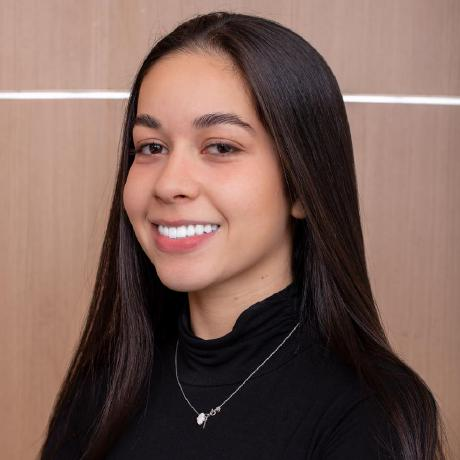
\includegraphics[
                        width=4.20cm,
                        height=4.20cm,
                        keepaspectratio
                    ]{profile.jpg}%
                }
            }
            {
                \fcolorbox{line}{soft}{
                    \parbox[c][4.20cm][c]{4.20cm}{
                        \centering

                        \color{muted}

                        \Large
                        \faUser

                        \par\vspace{0.10cm}

                        \scriptsize
                        profile.jpg
                    }
                }
            }

        \end{minipage}

        \end{tabularx}
    }
    {
        \begin{tabularx}{\linewidth}{
            @{}
            >{\raggedright\arraybackslash}X
            >{\raggedright\arraybackslash}p{6.2cm}
            @{}
        }

        \begin{minipage}[c]{\linewidth}

            \HeaderName{#1}{#2}

        \end{minipage}

        &

        \begin{minipage}[c]{\linewidth}

            \HeaderContacts{#3}{#5}

        \end{minipage}

        \end{tabularx}
    }

    \vspace{0.10cm}

    {\color{primary}
    \rule{\linewidth}{1.15pt}}

    \vspace{0.10cm}
}

% =========================================================
% COMPANY DESCRIPTOR (one line of context under a role)
% =========================================================
\newcommand{\roleinfo}[1]{
    {\small\itshape\color{muted}#1}

    \vspace{-0.03cm}
}

% =========================================================
% =========================================================
% ENGLISH VERSION
% =========================================================
% =========================================================

\newcommand{\EnglishCV}{

% =========================================================
% HEADER
% =========================================================
\CVHeader
{MOBILE SOFTWARE ENGINEER \;|\; FLUTTER DEVELOPER}
{Flutter \;•\; Dart \;•\; Android \& iOS \;•\; 4+ years in production}
{\LocationEN}
{nophoto}
{\WorkModeEN}

% =========================================================
% SUMMARY
% =========================================================
\cvsection{\faUser}{Professional Summary}

{\small
\justifying
Mobile Software Engineer specialized in \textbf{Flutter and Dart}, with 4+
years shipping production apps for Android and iOS and a B.Sc. in Systems
Engineering from UFMG. At \textbf{R10 Score} (1M+ Google Play downloads),
built real-time, high-traffic features end to end, such as the 2026 World Cup
experience and the live bet wall. At Prime Results, turned a white-label app
for 8 client companies into one flavor-based codebase. Strong in
Clean Architecture, BLoC/Cubit, real-time data (WebSocket, Protobuf) and testing;
also delivers with React, NestJS, Java and Spring.
}

% =========================================================
% CORE SKILLS
% =========================================================
\cvsection{\faCode}{Core Technical Skills}

\skillline
{Mobile}
{Flutter, Dart, Android, iOS, Kotlin, Swift, platform channels, flavors /
white-label, adaptive tablet UI, In-App Purchases, React Native}

\skillline
{State \& Architecture}
{BLoC, Cubit, Freezed, GoRouter, Clean Architecture, SOLID, dependency
injection, modular monorepo}

\skillline
{APIs \& Real-Time}
{REST APIs, JSON, Protobuf, WebSocket, Swagger / OpenAPI}

\skillline
{Firebase \& Data}
{Firebase, Crashlytics, Analytics, Realtime Database, feature flags, SQL,
PostgreSQL}

\skillline
{Web \& Backend}
{React, TypeScript, NestJS, Prisma, Java, Spring}

\skillline
{Quality \& Delivery}
{Unit, Widget \& Integration Testing (bloc\_test, mocktail), Code Review, CI/CD, GitHub
Actions, Codemagic, Git, Azure DevOps, Figma, Scrum, AI-assisted development
(Claude Code)}

\skillline
{Languages}
{Portuguese (native), English (professional working proficiency, B2 · TOEFL)}

% =========================================================
% EXPERIENCE
% =========================================================
\cvsection{\faBriefcase}{Professional Experience}

\experience
{Full Stack Developer | Mobile (Flutter)}
{OTG Ventures \;·\; R10 Score}
{Jun 2025 -- Sep 2026}
{
\roleinfo{Live football scores and statistics app \;·\; 1M+ Google
Play downloads \;·\; 11-package Flutter
monorepo}

\begin{itemize}

    \item
    Delivered the \textbf{2026 World Cup experience} (bracket, group tables,
    Favorite Team vote, match guesses and CMS-driven content) in time for the
    tournament's fixed start, joined by
    \textbf{22\% of all accounts}.

    \item
    Main mobile developer on \textbf{Notified Bet}: a live bet wall with
    drag-and-drop ordering saved on the backend (optimistic updates with
    rollback) and live status over \textbf{WebSocket}.

    \item
    \textbf{Unblocked Google Play publishing} after the 2026 target-API
    deadline (targetSdk 36, Play Billing Library 8.0.0), protecting In-App
    Purchase subscription revenue.

    \item
    Brought the test suite back to green, fixing two production bugs along the
    way, and tracked down an intermittent freeze in match statistics; one of
    the team's most active contributors, with \textbf{500+ merged PRs} and
    570+ code reviews.

    \item
    Built on \textbf{WebSocket (Protobuf and JSON) and REST}, with
    \textbf{Firebase} feature flags and Crashlytics; also contributed full stack
    to \textbf{OTG Partners}, the group's affiliate-commission platform
    (\textbf{React, NestJS}, Prisma, PostgreSQL).
\end{itemize}
}

\experience
{Mobile Developer}
{Prime Results}
{May 2022 -- May 2025}
{
\roleinfo{Intern from May 2022, Mobile Developer from Feb 2023 \;·\; white-label app for the
field and point-of-sale teams of 8 client companies \;·\; Android \& iOS}

\begin{itemize}

    \item
    Consolidated a \textbf{white-label app for 8 client companies}, kept on
    separate cherry-picked branches, into \textbf{one codebase with Flutter
    flavors}, so every fix ships to all clients from a single main branch.

    \item
    Adjusted and improved \textbf{phone and tablet layouts} across the app,
    used by field and point-of-sale teams.

    \item
    Delivered features end to end, from \textbf{Figma} to \textbf{REST API}
    integration and releases on \textbf{Google Play and the App Store}, and contributed to \textbf{Java and Spring}
    services and \textbf{React} web projects.
\end{itemize}
}

\experience
{Mobile Developer -- Freelance}
{Upbeat Studio \;·\; Drum Coach app -- Germany (remote)}
{Mar 2025 -- Apr 2025}
{
\begin{itemize}

    \item
    Built an interactive \textbf{Flutter and Dart} app for learning and
    practicing drums, working remotely and autonomously with an international
    team in English.
\end{itemize}
}

\experience
{Programming Instructor (Volunteer)}
{Garotas Aplicadas Project -- AVEC | Centro Universitário Una}
{Jan 2025 -- Aug 2026}
{
\begin{itemize}

    \item
    Taught theory and hands-on programming classes to public
    high-school girls in Belo Horizonte, in a social initiative to
    widen female participation in technology.
\end{itemize}
}

\experience
{Business Analyst \& Front-End Developer}
{iJunior}
{Mar 2022 -- May 2022}
{
\begin{itemize}

    \item
    Gathered requirements with clients and the sales team and built custom
    apps and websites with \textbf{React Native} for organizations across
    different sectors, using \textbf{Scrum and Kanban}.
\end{itemize}
}

\experience
{Systems Analyst}
{Interact Place}
{Oct 2021 -- Jan 2022}
{
\begin{itemize}

    \item
    Helped build an interactive mobile exhibition guide for
    \textbf{Palácio das Artes}, one of Belo Horizonte's major cultural
    institutions, where QR codes connect visitors to artwork information.
\end{itemize}
}

% =========================================================
% EDUCATION
% =========================================================
\cvsection{\faGraduationCap}{Education \& Certifications}

\education
{Bachelor's Degree in Systems Engineering}
{Federal University of Minas Gerais -- UFMG}
{2020 -- 2026}
{}

\skillline
{Certifications}
{TOEFL (English, B2) \;·\; CCAA English course (2008 -- 2019) \;·\; Google
Play Academy -- Store Listing Certificate}

}


% =========================================================
% =========================================================
% PORTUGUESE VERSION
% =========================================================
% =========================================================

\newcommand{\PortugueseCV}{

% =========================================================
% HEADER
% =========================================================
\CVHeader
{ENGENHEIRA DE SOFTWARE MOBILE \;|\; DESENVOLVEDORA FLUTTER}
{Flutter \;•\; Dart \;•\; Android e iOS \;•\; 4+ anos em produção}
{\LocationPT}
{photo}
{\WorkModePT}

% =========================================================
% SUMMARY
% =========================================================
\cvsection{\faUser}{Resumo Profissional}

{\small
\justifying
Engenheira de Software Mobile especializada em \textbf{Flutter e Dart}, com
mais de 4 anos entregando apps em produção para Android e iOS, formada em
Engenharia de Sistemas pela UFMG. No \textbf{R10 Score} (mais de 1 milhão de
downloads no Google Play), desenvolvi de ponta a ponta funcionalidades em tempo
real e de alto tráfego, como a experiência da Copa do Mundo 2026 e o mural de
apostas ao vivo. Na Prime Results, transformei um app white-label de 8 empresas
clientes em um único código com flavors. Forte em Clean Architecture,
BLoC/Cubit, dados em tempo real (WebSocket, Protobuf) e testes; também atuo com
React, NestJS, Java e Spring.
}

% =========================================================
% CORE SKILLS
% =========================================================
\cvsection{\faCode}{Competências Técnicas}

\skillline
{Mobile}
{Flutter, Dart, Android, iOS, Kotlin, Swift, platform channels, flavors /
white-label, UI adaptativa para tablet, compras in-app, React Native}

\skillline
{Estado \& Arquitetura}
{BLoC, Cubit, Freezed, GoRouter, Clean Architecture, SOLID, injeção de
dependência, monorepo modular}

\skillline
{APIs \& Tempo Real}
{APIs REST, JSON, Protobuf, WebSocket, Swagger / OpenAPI}

\skillline
{Firebase \& Dados}
{Firebase, Crashlytics, Analytics, Realtime Database, feature flags, SQL,
PostgreSQL}

\skillline
{Web \& Backend}
{React, TypeScript, NestJS, Prisma, Java, Spring}

\skillline
{Qualidade \& Entrega}
{Testes Unitários, de Widget e de Integração (bloc\_test, mocktail), Code Review, CI/CD,
GitHub Actions, Codemagic, Git, Azure DevOps, Figma, Scrum, desenvolvimento
assistido por IA (Claude Code)}

\skillline
{Idiomas}
{Português (nativo), Inglês (proficiência profissional, B2 · TOEFL)}

% =========================================================
% EXPERIENCE
% =========================================================
\cvsection{\faBriefcase}{Experiência Profissional}

\experience
{Desenvolvedora Full Stack | Mobile (Flutter)}
{OTG Ventures \;·\; R10 Score}
{Jun 2025 -- Set 2026}
{
\roleinfo{App de placares e estatísticas de futebol ao vivo \;·\;
mais de 1 milhão de downloads no Google Play \;·\; monorepo Flutter com 11 pacotes}

\begin{itemize}

    \item
    Entreguei a \textbf{experiência da Copa do Mundo 2026} (chaveamento,
    tabela de grupos, votação do Time do Coração, palpites e conteúdo via CMS)
    a tempo do início do torneio, com adesão de
    \textbf{22\% de todas as contas}.

    \item
    Principal desenvolvedora mobile da \textbf{Aposta Notificada}: mural de apostas ao vivo
    com reordenação por drag-and-drop salva no backend (atualização otimista
    com rollback) e status em tempo real via \textbf{WebSocket}.

    \item
    \textbf{Desbloqueei a publicação no Google Play} após o prazo de target
    API de 2026 (targetSdk 36, Play Billing Library 8.0.0), protegendo a
    receita das assinaturas (compras in-app).

    \item
    Recuperei a suíte de testes, corrigindo dois bugs de produção no caminho,
    e rastreei um travamento intermitente nas estatísticas das partidas; estou
    entre as pessoas mais ativas do time, com \textbf{mais de 500 PRs}
    mergeados e mais de 570 code reviews.

    \item
    Desenvolvi sobre \textbf{WebSocket (Protobuf e JSON) e REST}, com
    feature flags no \textbf{Firebase} e Crashlytics; atuei também full stack
    no \textbf{OTG Partners}, plataforma de comissões de afiliados do grupo
    (\textbf{React, NestJS}, Prisma, PostgreSQL).
\end{itemize}
}

\experience
{Desenvolvedora Mobile}
{Prime Results}
{Mai 2022 -- Mai 2025}
{
\roleinfo{Estagiária desde mai 2022, Desenvolvedora Mobile desde fev 2023 \;·\; app
white-label para equipes de campo e de ponto de venda de 8 empresas clientes}

\begin{itemize}

    \item
    Consolidei um \textbf{app white-label de 8 empresas clientes}, mantido em
    branches separadas sincronizadas por cherry-pick, em \textbf{um único
    código com flavors do Flutter}, para que cada correção chegue a todos os
    clientes a partir de uma única branch principal.

    \item
    Ajustei e melhorei \textbf{layouts para celular e tablet} em todo o app,
    usado por equipes de campo e de ponto de venda.

    \item
    Entreguei funcionalidades de ponta a ponta, do \textbf{Figma} à
    integração com \textbf{APIs REST} e à publicação no \textbf{Google Play e na App Store}, e contribuí em serviços
    \textbf{Java e Spring} e em projetos web com \textbf{React}.
\end{itemize}
}

\experience
{Desenvolvedora Mobile -- Freelancer}
{Upbeat Studio \;·\; app Drum Coach -- Alemanha (remoto)}
{Mar 2025 -- Abr 2025}
{
\begin{itemize}

    \item
    Desenvolvi um app interativo em \textbf{Flutter e Dart} para aprender e
    praticar bateria, em trabalho remoto e autônomo com uma equipe
    internacional, em inglês.
\end{itemize}
}

\experience
{Instrutora de Programação (Voluntária)}
{Projeto Garotas Aplicadas -- AVEC | Centro Universitário Una}
{Jan 2025 -- Ago 2026}
{
\begin{itemize}

    \item
    Dei aulas teóricas e práticas de programação para estudantes do ensino
    médio da rede pública de Belo Horizonte, em uma iniciativa social para
    ampliar a participação feminina na tecnologia.
\end{itemize}
}

\experience
{Analista de Negócios \& Desenvolvedora Front-End}
{iJunior}
{Mar 2022 -- Mai 2022}
{
\begin{itemize}

    \item
    Levantei requisitos com clientes e com a equipe comercial e desenvolvi
    aplicações e websites personalizados com \textbf{React Native} para
    organizações de diferentes segmentos, com \textbf{Scrum e Kanban}.
\end{itemize}
}

\experience
{Analista de Sistemas}
{Interact Place}
{Out 2021 -- Jan 2022}
{
\begin{itemize}

    \item
    Participei do desenvolvimento de um guia mobile interativo de exposições
    para o \textbf{Palácio das Artes}, uma das principais instituições
    culturais de Belo Horizonte, em que QR Codes conectam os visitantes a
    informações sobre as obras.
\end{itemize}
}

% =========================================================
% EDUCATION
% =========================================================
\cvsection{\faGraduationCap}{Formação \& Certificações}

\education
{Bacharelado em Engenharia de Sistemas}
{Universidade Federal de Minas Gerais -- UFMG}
{2020 -- 2026}
{}

\skillline
{Certificações}
{TOEFL (inglês, B2) \;·\; Curso de inglês CCAA (2008 -- 2019) \;·\; Google
Play Academy -- Store Listing Certificate}

}

% =========================================================
% LANGUAGE-SPECIFIC PDF METADATA
% =========================================================
\newcommand{\MetadataEN}{
    \hypersetup{
        pdftitle={Beatriz Vocurca Frade - Mobile Software Engineer - Flutter Developer},
        pdfsubject={Mobile Software Engineering, Flutter and Software Development Resume},
        pdflang={en-US}
    }
}

\newcommand{\MetadataPT}{
    \hypersetup{
        pdftitle={Beatriz Vocurca Frade - Engenheira de Software Mobile - Desenvolvedora Flutter},
        pdfsubject={Currículo de Engenharia de Software Mobile, Flutter e Desenvolvimento de Software},
        pdflang={pt-BR}
    }
}

\ifthenelse{\equal{\CVLang}{pt}}
{\MetadataPT}
{\MetadataEN}


% =========================================================
% DOCUMENT
% =========================================================
\begin{document}

\ifthenelse{\equal{\CVLang}{en}}
{
    \EnglishCV
}
{
    \ifthenelse{\equal{\CVLang}{pt}}
    {
        \PortugueseCV
    }
    {
        % Bilingual: English first, Portuguese after a page break
        \EnglishCV

        \newpage

        \PortugueseCV
    }
}

\end{document}
